\documentclass[12pt]{article}
\usepackage[margin=2.5cm]{geometry}
\usepackage{enumerate}
\usepackage{amsfonts}
\usepackage{amsmath}
\usepackage{fancyhdr}
\usepackage{amsmath}
\usepackage{amssymb}
\usepackage{amsthm}
\usepackage{mdframed}
\usepackage{graphicx}
\usepackage{subcaption}
\usepackage{adjustbox}
\usepackage{listings}
\usepackage{xcolor}
\usepackage{courier}
\usepackage[utf]{kotex}
\usepackage{hyperref}
\usepackage{soul}

\definecolor{codegreen}{rgb}{0,0.6,0}
\definecolor{codegray}{rgb}{0.5,0.5,0.5}
\definecolor{codepurple}{rgb}{0.58,0,0.82}
\definecolor{backcolour}{rgb}{0.95,0.95,0.92}

\lstdefinestyle{mystyle}{
    backgroundcolor=\color{backcolour},
    commentstyle=\color{codegreen},
    keywordstyle=\color{magenta},
    numberstyle=\tiny\color{codegray},
    stringstyle=\color{codepurple},
    basicstyle=\ttfamily\footnotesize,
    breakatwhitespace=false,
    breaklines=true,
    captionpos=b,
    keepspaces=true,
    numbers=left,
    numbersep=5pt,
    showspaces=false,
    showstringspaces=false,
    showtabs=false,
    tabsize=1
}

\lstset{style=mystyle}

\pagestyle{fancy}
\renewcommand{\headrulewidth}{0.4pt}
\lhead{CSC 369}
\rhead{Midterm 4 Notes}

\begin{document}
\title{CSC 369 Midterm 4 Notes}

\section{Exam Related Questions and Tips}

\begin{itemize}
    \item What is hard link? What is soft link? What are the differences between the two?
    \item I wonder how system call for reading file/directory works in UNIX. Does it check for bitmap?
    \item I wonder how system call for deleting file/directory works in UNIX
    \item I wonder how system call for creatubg file/directory works in UNIX
    \item Learned that
    \begin{itemize}
        \item Missing Inode Bitmap - multiple file paths may point to same inode
    \end{itemize}
\end{itemize}

\section{Files and Directories}
\subsection{File}
\begin{itemize}
    \item Is a linear array of bytes, which you can read or write
    \item Low-level name called \textbf{i-number}
    \begin{itemize}
        \item inode also has a low-level name \textbf{i-number}
        \item File is an inode
    \end{itemize}
\end{itemize}

\subsection{Directory}
\begin{itemize}
    \item Is like a file
    \item Also has a low-level name \textbf{i-number}
    \begin{itemize}
        \item Directory is also an inode
    \end{itemize}
    \item Provides logical structure to file systems
    \item Contains a list of (user-readable name, low-level name)

    \bigskip

    \underline{\textbf{Example}}

    \bigskip

    File with low-level name `10', and user-readible name `foo'.

    \bigskip

    Directory has entry (`foo', 10) in list (in a data block) that points to the file.
\end{itemize}

\subsection{Directory Implementation}
\begin{itemize}
    \item Option 1: List
    \begin{itemize}
        \item Is simple list of file names and pointers to file metadata
        \item Requires a linear search to find entries
        \item Easy to implement and slow to execute (Not a good option)
    \end{itemize}
    \item Option 2: Hash Table
    \begin{itemize}
        \item Creates a list of file info structures
        \item Has file name to get a pointer to the file name info structure in the list
        \item Takes space
    \end{itemize}
\end{itemize}

\section{File API}
\begin{itemize}
    \item \texttt{open} (create/access file)
    \begin{itemize}
        \item Is a system call
        \item Reads target inode into memory (when loading)
        \item Does three things on creation

        \begin{enumerate}[1)]
            \item make structure (inode) that racks all relevant information about file
            \item link human readible name to the file, and put that link to a directory
            \item increment \textbf{reference count} in inode
        \end{enumerate}

        \item \textbf{Syntax:}

        \bigskip

        \texttt{int fd = open("foo". O\_CREAT|O\_WRONLY|O\_TRUNC, S\_IRUSR|S\_IWUSR)}

        \bigskip

        \begin{itemize}
            \item \texttt{O\_CREAT} - Creates file "foo" if does not exist
            \item \texttt{O\_WRONLY} - Open file for writing only (default)
            \item \texttt{O\_TRUNC} - Overwrites existing file \color{red}Need example/Clarification\color{black}
            \item Can have multiple flags
        \end{itemize}
        \item Returns \textbf{file descriptor} or \texttt{fd} for short

        \begin{itemize}
            \item Is an integer
            \item Is used to access a file
            \item Is \underline{private} per process
            \item Can be used to \texttt{read()} and \texttt{write()} files
        \end{itemize}

        \bigskip

        \underline{\textbf{Example}}

        \bigskip

        \begin{center}
        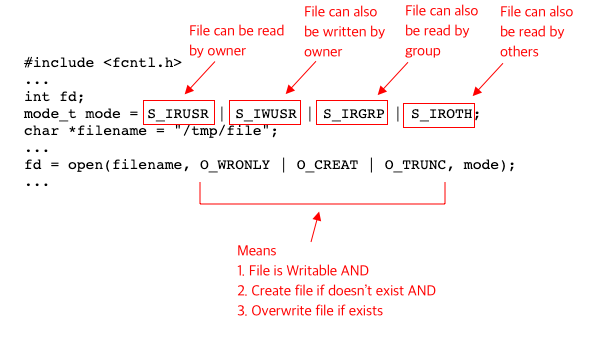
\includegraphics[width=\linewidth]{../images/midterm_4_solution_2.png}
        \end{center}

        \item Amount of I/O generated by \texttt{open()} is proportional to length
        of pathname (wait. How is I/O involved in open()?)

        \bigskip

    \end{itemize}

    \item \texttt{read} (read file)
    \begin{itemize}
        \item Is a system call
        \item \textbf{Syntax:}

        \bigskip

        \texttt{ssize\_t read (int fd, void *buf, size\_t count)}

        \bigskip

        \begin{itemize}
            \item \texttt{fd} - file descriptor (from \texttt{open()})
            \item \texttt{buf} - container for the read data
            \item \texttt{count} - number of bytes to read
        \end{itemize}
        \item Returns number of bytes read, if successful
        \item Returns 0 if is at, or past the end of file

        \bigskip

        \underline{\textbf{Example}}

        \bigskip

        \begin{center}
        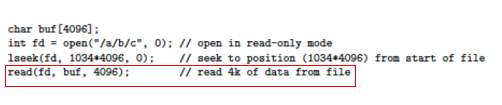
\includegraphics[width=\linewidth]{../images/midterm_4_solution_3.png}
        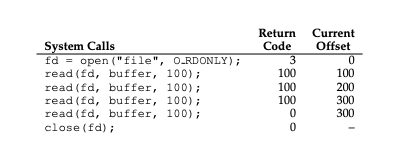
\includegraphics[width=\linewidth]{../images/midterm_4_solution_5.png}
        \end{center}

    \end{itemize}

    \item \texttt{write} (write file)

    \begin{itemize}
        \item Is a system call
        \item Writes data out of a buffer
        \item \textbf{Syntax:}

        \bigskip

        \texttt{ssize\_t write (int fd, const void * buf, size\_t nbytes)}

        \bigskip

        \begin{itemize}
            \item \texttt{fd} - file descriptor
            \item \texttt{buf} - A pointer to a buffer to write to file
            \item \texttt{nbytes} - number of bytes to write. If smaller than buffer, the output is truncated
        \end{itemize}
    \end{itemize}

    \bigskip

    \underline{\textbf{Example}}

    \bigskip

    \begin{center}
    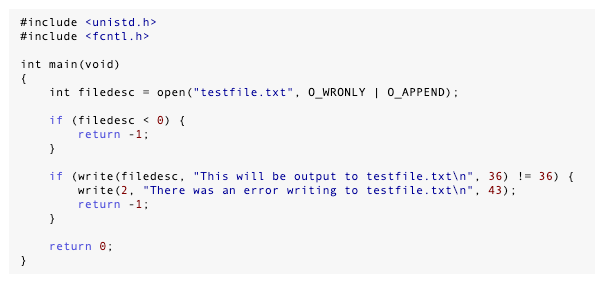
\includegraphics[width=\linewidth]{../images/midterm_4_solution_4.png}
    \end{center}

    \item \texttt{lseek}

    \begin{itemize}
        \item Reads or write to a specific offset within a file
        \item \textbf{Syntax:}

        \bigskip

        \texttt{off\_t lseek (int fd, off\_t offset, int whence)}

        \bigskip

        \begin{itemize}
            \item \texttt{fd} - file descriptor
            \item \texttt{offset} - the offset of pointer within file (in bytes)
            \item \texttt{whence} - the method of offset

            \bigskip

            \quad \texttt{SEEK\_SET}  - offset from the start of file (absolute)

            \quad \texttt{SEEK\_CUR} - offset from current location + offset bytes (relative)

            \quad \texttt{SEEK\_END} - offset from the end of file
        \end{itemize}

        \item Returns offset amount (in bytes) from the \underline{beginning} of file
        \item Returns -1 if error
    \end{itemize}

    \bigskip

    \underline{\textbf{Example}}

    \begin{center}
    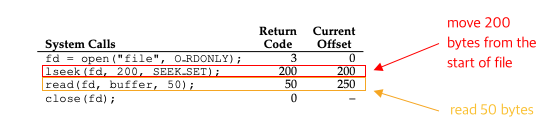
\includegraphics[width=\linewidth]{../images/midterm_4_solution_7.png}
    \end{center}

    \item \texttt{rename} (update file name)

    \begin{itemize}
        \item Is a system call
        \item Changes the name of file
        \item Is \textbf{atomic} (after crash, it will be either old or new, but not in-between)
        \item \textbf{Syntax:} \texttt{int rename(const char *old, const char *new)}

        \begin{itemize}
            \item \texttt{old} - name of old file
            \item \texttt{new} - name of new file
        \end{itemize}

        \item Returns 0 if successful
        \item Returns -1 if error
    \end{itemize}

    \bigskip

    \underline{\textbf{Example}}

    \begin{center}
    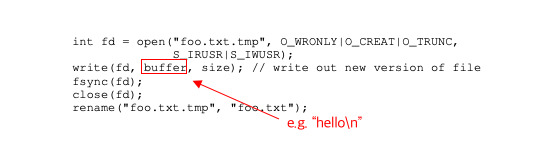
\includegraphics[width=\linewidth]{../images/midterm_4_solution_8.png}
    \end{center}

    \item \texttt{stat} (get file info)

    \begin{itemize}
        \item displays metadata of a certain file stored in \textbf{inode}
        \item \textbf{Syntax:} \texttt{int stat(const char *path, struct stat *buf)}

        \begin{itemize}
            \item \texttt{path} - file descriptor of file that's being inquired
            \item \texttt{buf} - A \texttt{stat} structure where data about the file will be stored (see below)

            \bigskip

            \begin{center}
            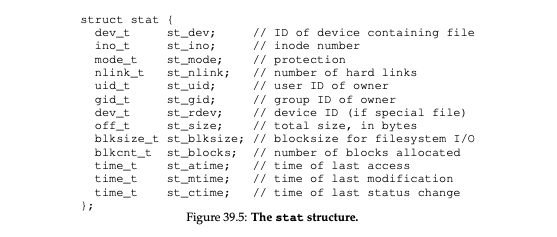
\includegraphics[width=\linewidth]{../images/midterm_4_solution_9.png}
            \end{center}
        \end{itemize}
    \end{itemize}

    \bigskip

    \underline{\textbf{Example}}

    \begin{center}
    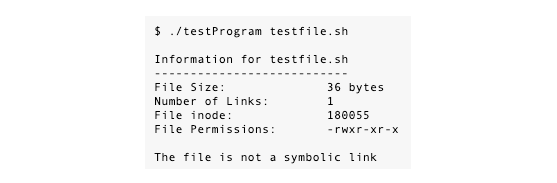
\includegraphics[width=\linewidth]{../images/midterm_4_solution_10.png}
    \end{center}

    \bigskip

    The result of above is:

    \begin{center}
    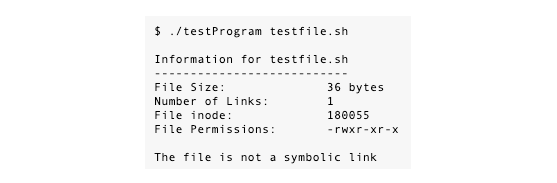
\includegraphics[width=\linewidth]{../images/midterm_4_solution_11.png}
    \end{center}

    \item \texttt{unlink} (removing file)

    \begin{itemize}
        \item Is a system call
        \item Removes a \underline{file} (including symbolic link) from the system
        \item \textbf{Syntax:} \texttt{int unlink(const char *pathname)}

        \begin{itemize}
            \item \texttt{pathname} - path to file
        \end{itemize}

        \item Returns 0 if successful
        \item Returns -1 if error
    \end{itemize}

    \bigskip

    \underline{\textbf{Example}}

    \begin{center}
    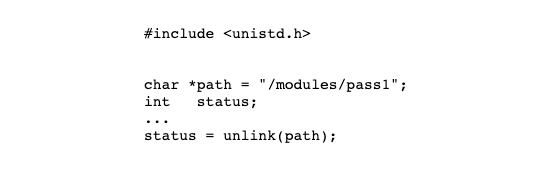
\includegraphics[width=\linewidth]{../images/midterm_4_solution_12.png}
    \end{center}

    \item \texttt{mkdir} (creating directory)

    \begin{itemize}
        \item Is a system call
        \item \textbf{Syntax:} \texttt{int mkdir(const char *path, mode\_t mode)}
        \begin{itemize}
            \item \texttt{path} - path of directory (including name)
            \item \texttt{mode} - permission group
        \end{itemize}
        \item Returns 0 if successful
        \item Returns -1 if error
        \item directories can never be written directly
        \begin{itemize}
            \item directory is in format called \textbf{File System Metadata}
            \item directory can \underline{only} be updated directly
        \end{itemize}
        \item creates two directories on creation \texttt{.} (current) and \texttt{..} (parent)
    \end{itemize}

    \bigskip

    \underline{\textbf{Example}}

    \begin{center}
    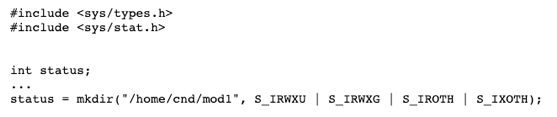
\includegraphics[width=\linewidth]{../images/midterm_4_solution_13.png}
    \end{center}

    \item \texttt{opendir, readdir, closedir} (reading directory)

    \begin{itemize}
        \item Are system calls
        \item Are under \texttt{$<$dirent.h$>$} library
        \item Requires \texttt{struct dirent} data structure

        \begin{center}
        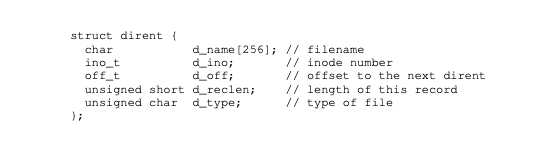
\includegraphics[width=\linewidth]{../images/midterm_4_solution_14.png}
        \end{center}

        \item \textbf{Syntax (opendir): } \texttt{DIR *opendir(const char *dirname)}
        \begin{itemize}
            \item \texttt{dirname} - directory path
            \item Returns a pointer to the directory stream
            \item The stream is positioned at \underline{the first entry} in the directory.
        \end{itemize}
        \item \textbf{Syntax (readdir): } \texttt{struct dirent *readdir(DIR *dirp);}
        \begin{itemize}
            \item \texttt{dirp} - directory stream
            \item Returns a pointer to a dirent structure representing the next directory entry in the directory stream
            \item Returns NULL on reaching the end of the directory stream
        \end{itemize}
        \item \textbf{Syntax (closedir): } \texttt{int closedir(DIR *dirp));}
        \begin{itemize}
            \item \texttt{dirp} - directory stream
            \item Returns 0 if successful
            \item Returns -1 otherwise
        \end{itemize}

        \bigskip

        \underline{\textbf{Example}}

        \bigskip

        \begin{center}
        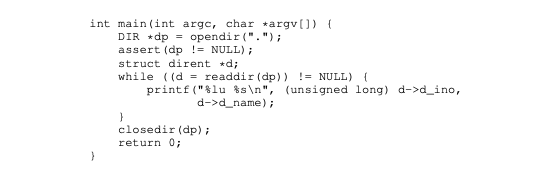
\includegraphics[width=\linewidth]{../images/midterm_4_solution_15.png}
        \end{center}

        \item \text{rmdir} (Deleting Directories)

        \begin{itemize}
            \item Removes a directory whose name is given by path
            \item Is performed only when directory is empty
            \item Is included in \texttt{$<$unistd.h$>$} library
            \item Fails if is symbolic link
            \item \textbf{Syntax:} \texttt{int rmdir(const char *path)}

            \begin{itemize}
                \item \texttt{path} - path of directory
            \end{itemize}
            \item Returns 0 if successful
            \item Returns -1 if error
        \end{itemize}

        \bigskip

        \underline{\textbf{Example}}

        \begin{center}
        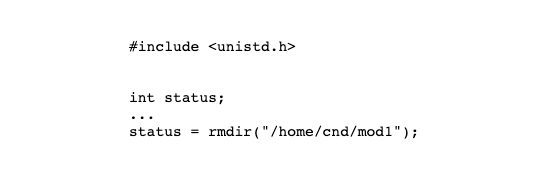
\includegraphics[width=\linewidth]{../images/midterm_4_solution_16.png}
        \end{center}

        \item \texttt{unlink} (Remove file)

        \begin{itemize}
            \item Remove a link to a file
            \item Is called \textbf{unlink} because it decrements \textbf{reference count} in inode
            \begin{itemize}
                \item Deletes file completely when reference count within the inode number is 0
            \end{itemize}
            \item \textbf{Syntax:}

            \bigskip
            \texttt{\#include $<$unistd.h$>$}

            \bigskip

            \texttt{int unlink(const char *pathname);}

            \bigskip

            \begin{itemize}
                \item \texttt{pathname} - pathname to file
            \end{itemize}
            \item Returns 0 if successful
            \item Returns -1 if error
            \item Is used by linux command \texttt{rm}
        \end{itemize}

        \bigskip

        \underline{\textbf{Example}}

        \begin{center}
        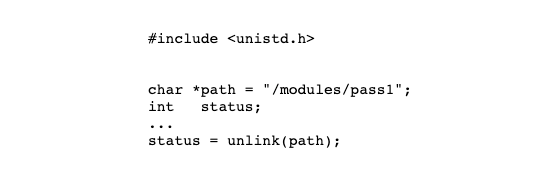
\includegraphics[width=\linewidth]{../images/midterm_4_solution_17.png}
        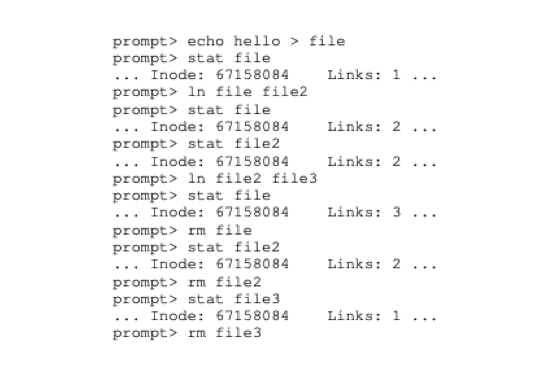
\includegraphics[width=\linewidth]{../images/midterm_4_solution_18.png}
        \end{center}
    \end{itemize}
\end{itemize}

\section{Symbolic Link:}


\begin{center}
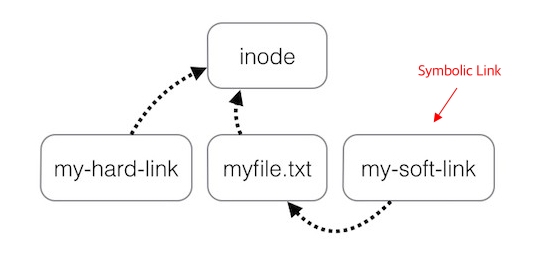
\includegraphics[width=0.8\linewidth]{../images/midterm_4_solution_48.png}
\end{center}

\begin{itemize}
    \item Is a pointer to a file
    \item \textbf{Syntax:} \texttt{ln -s \{source\} \{link\}}
    \item Is a shortcut (a special file) that reference to a file instead of inode value $^{[2]}$
    \item Can create symbolic links to directories
    \item Can create symbolic links across partitions
    \item Deleting the source file $\to$ Problem
    \begin{itemize}
        \item Inode of file is deleted when reference count is 0
        \item Creates a \textbf{dangling pointer}
    \end{itemize}

    \begin{center}
        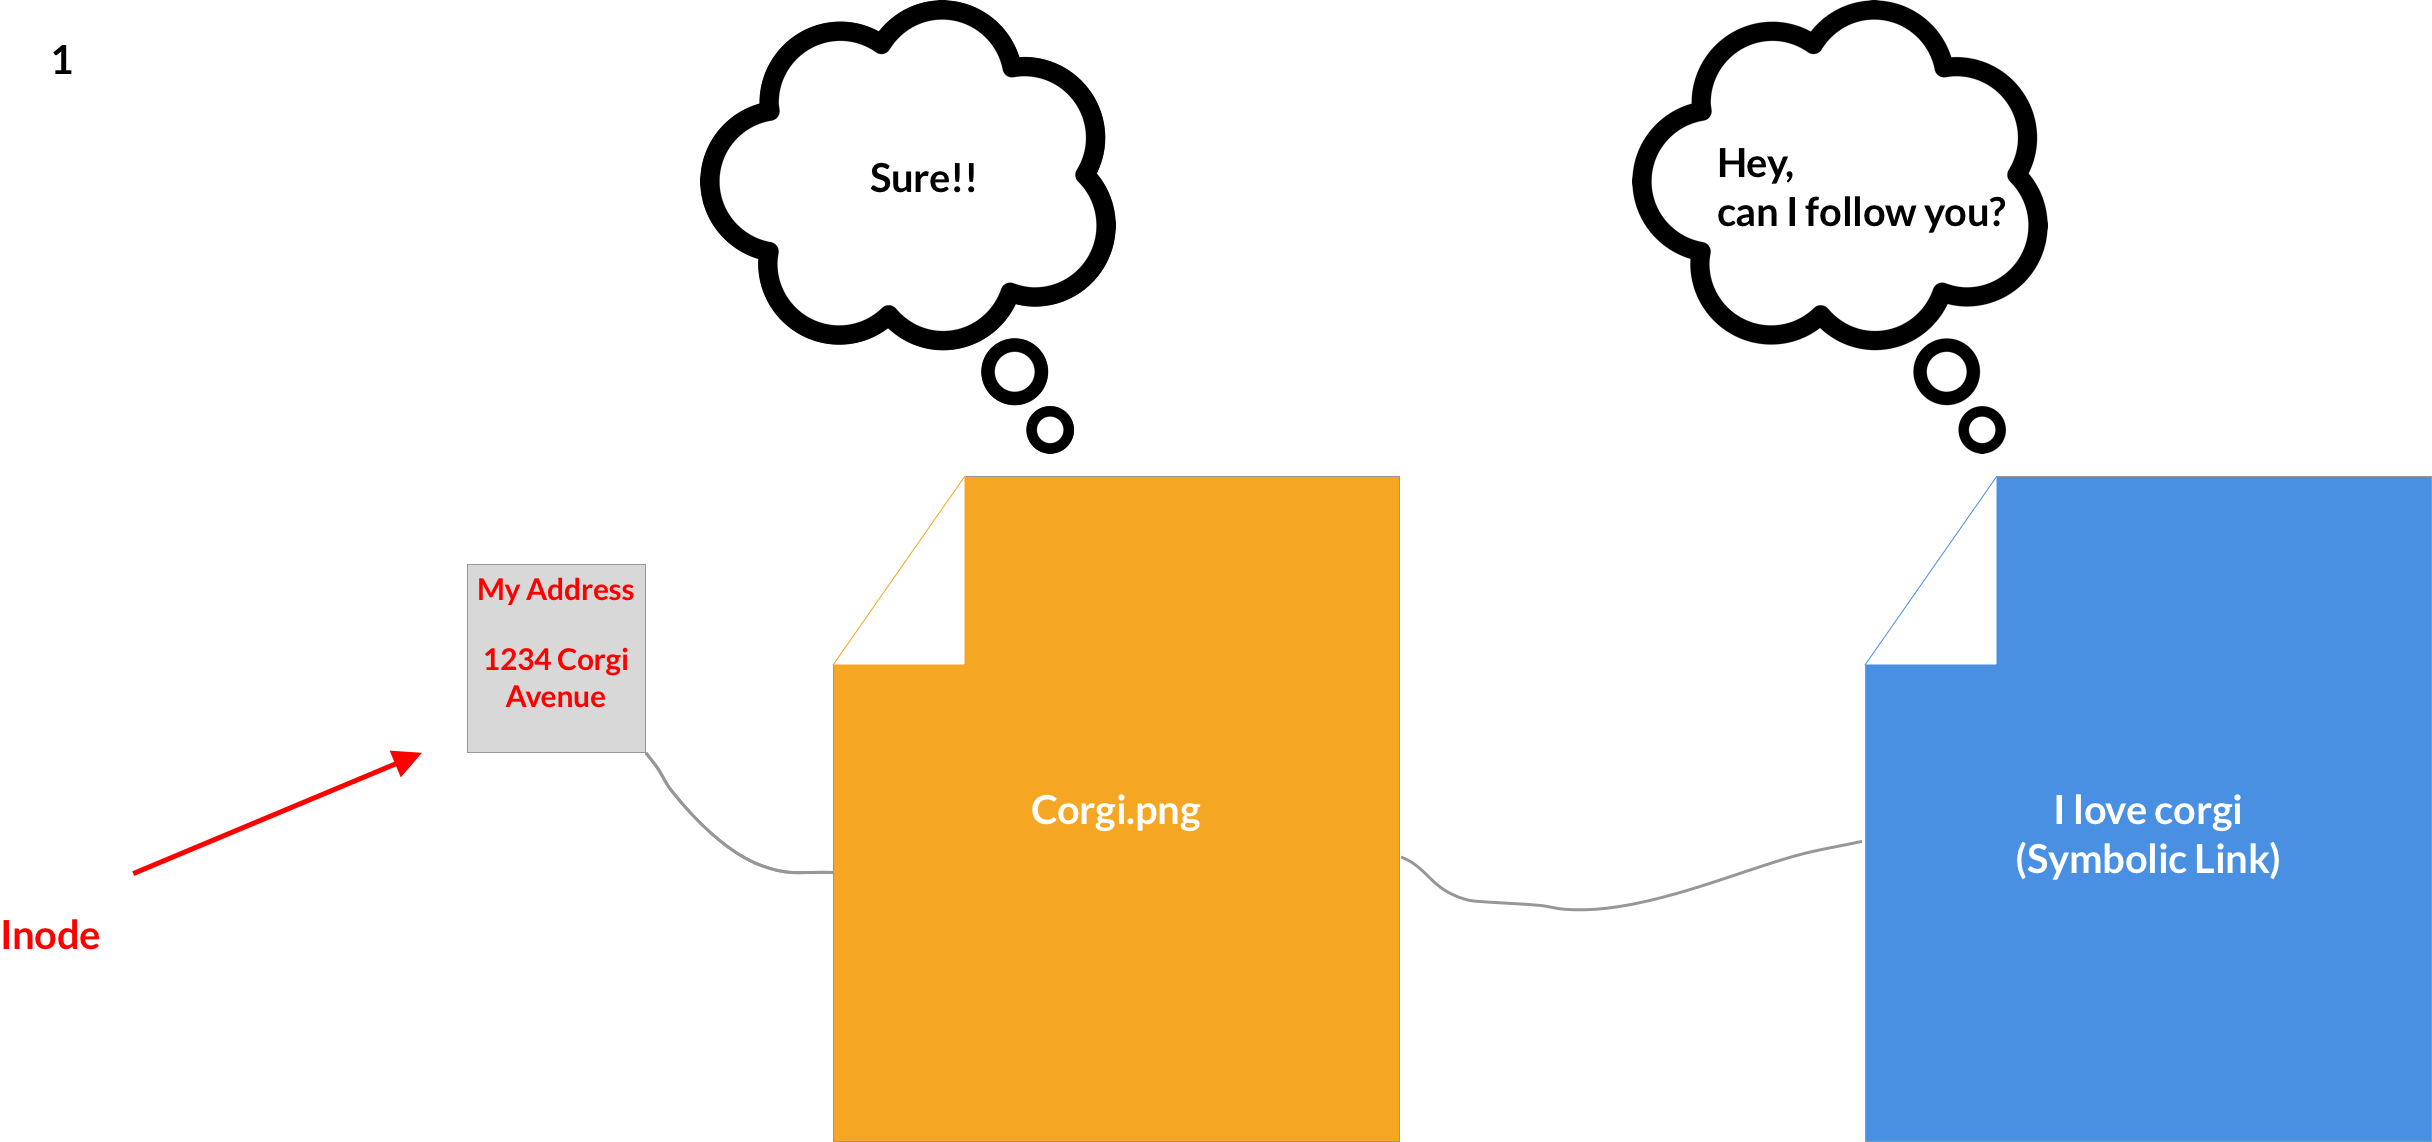
\includegraphics[width=0.8\linewidth]{../images/midterm_4_solution_19.png}
        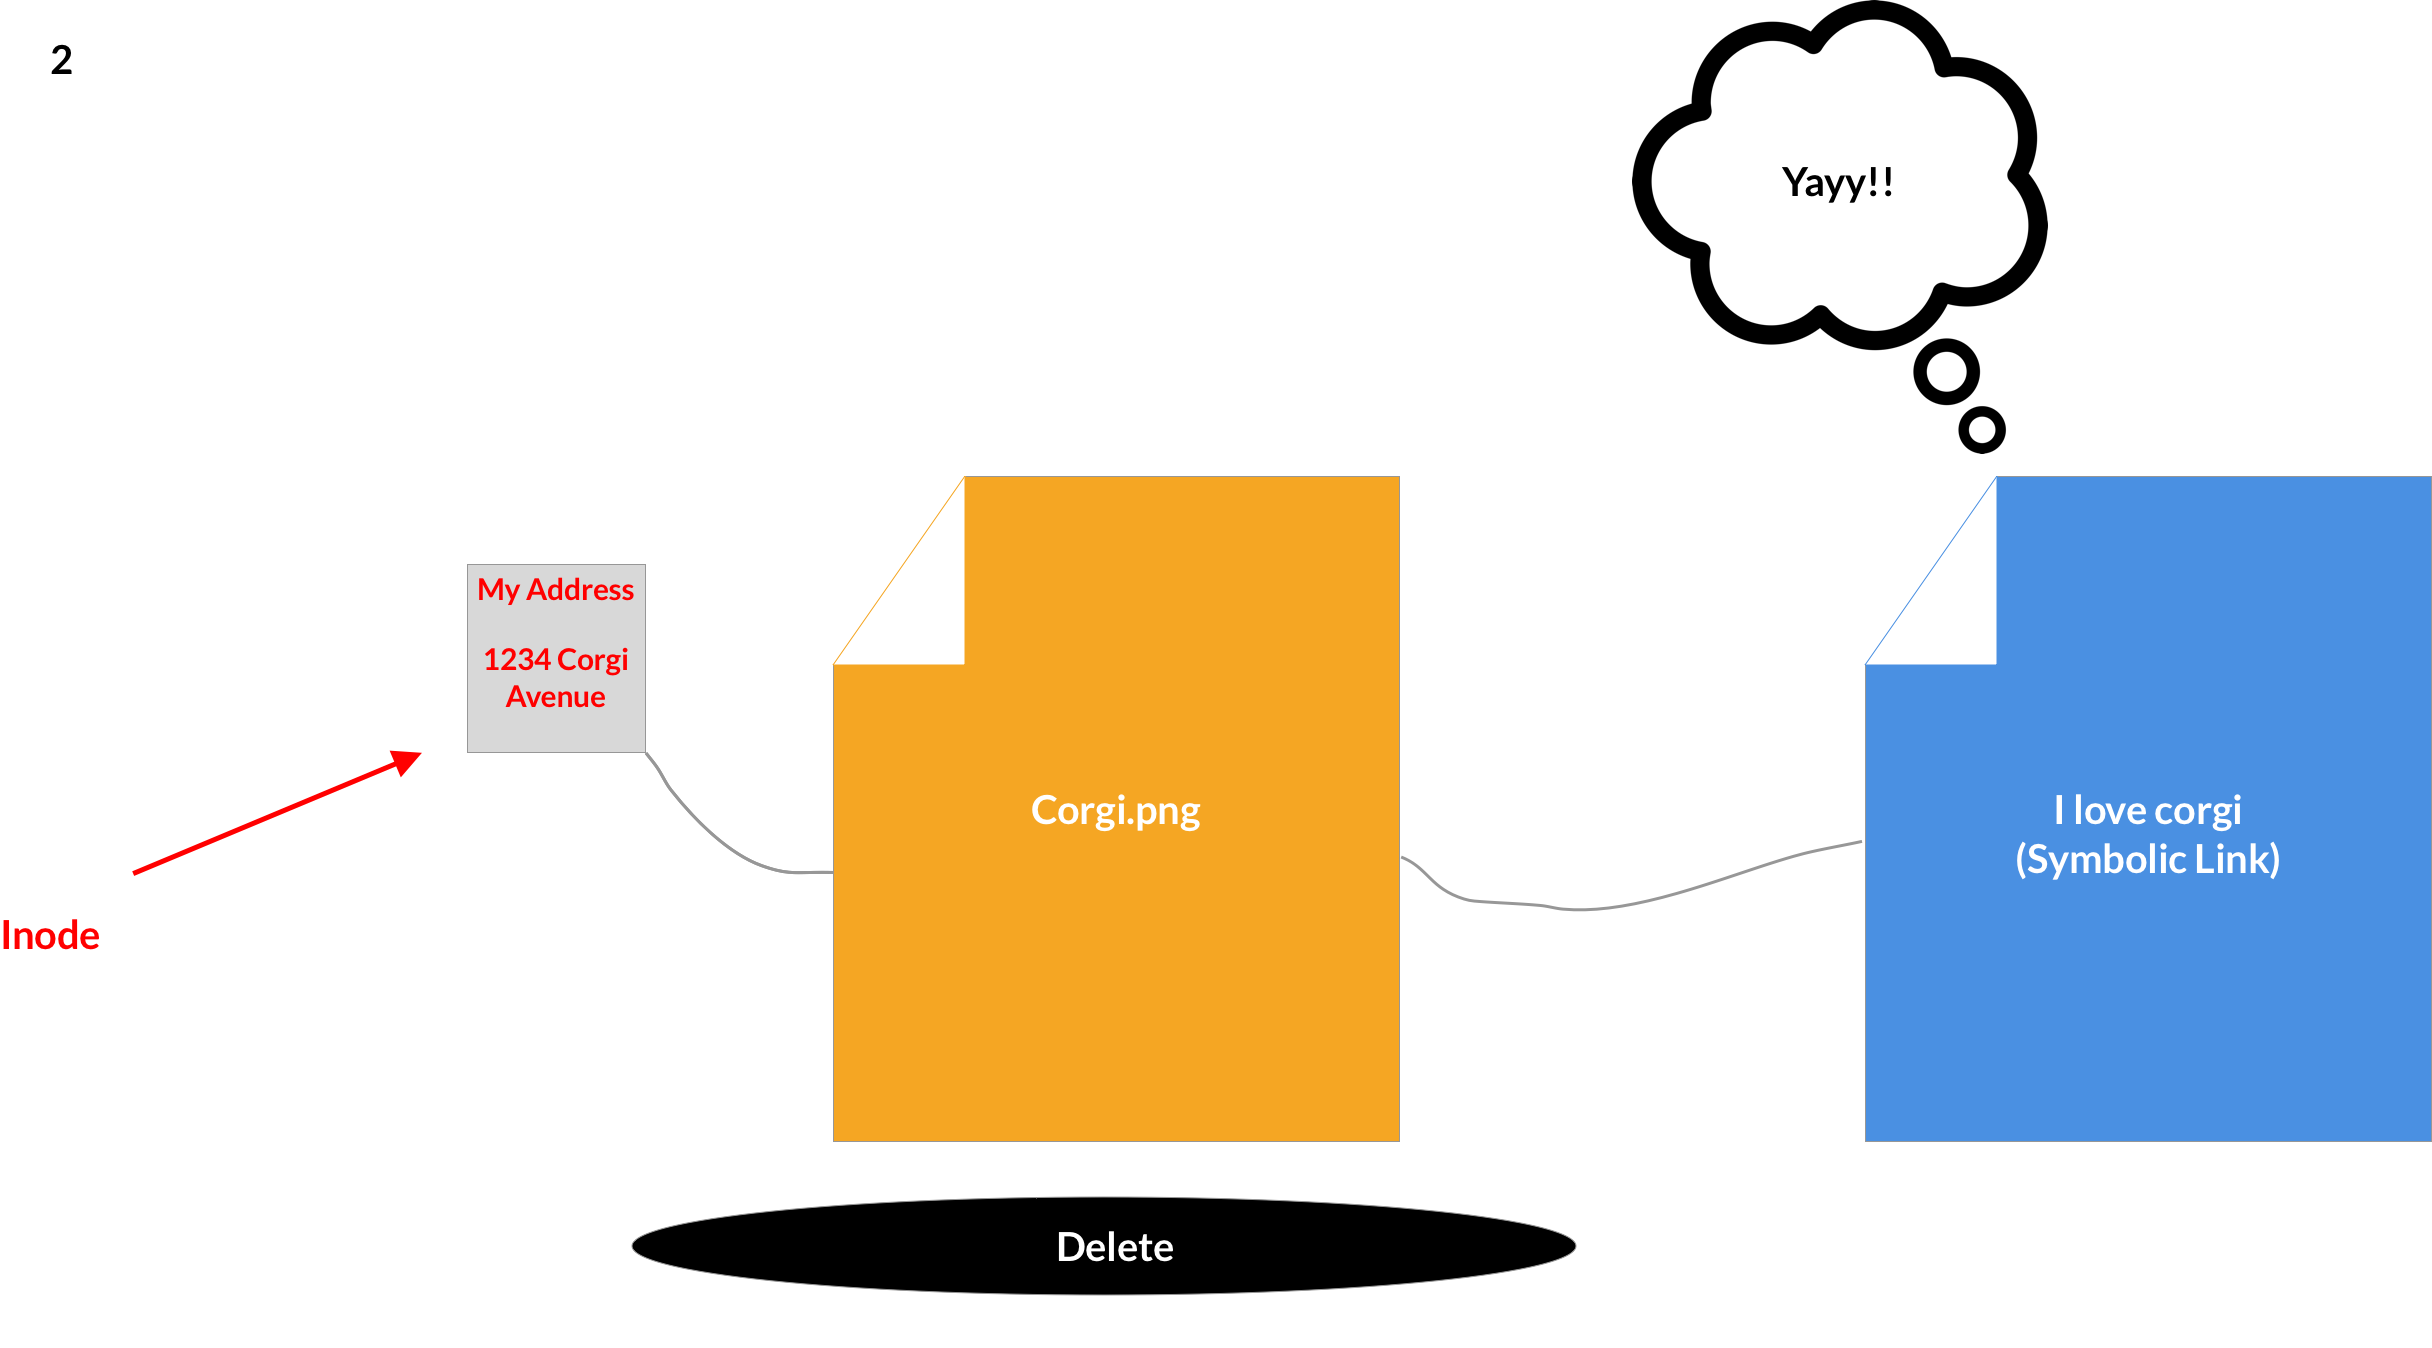
\includegraphics[width=0.8\linewidth]{../images/midterm_4_solution_20.png}
        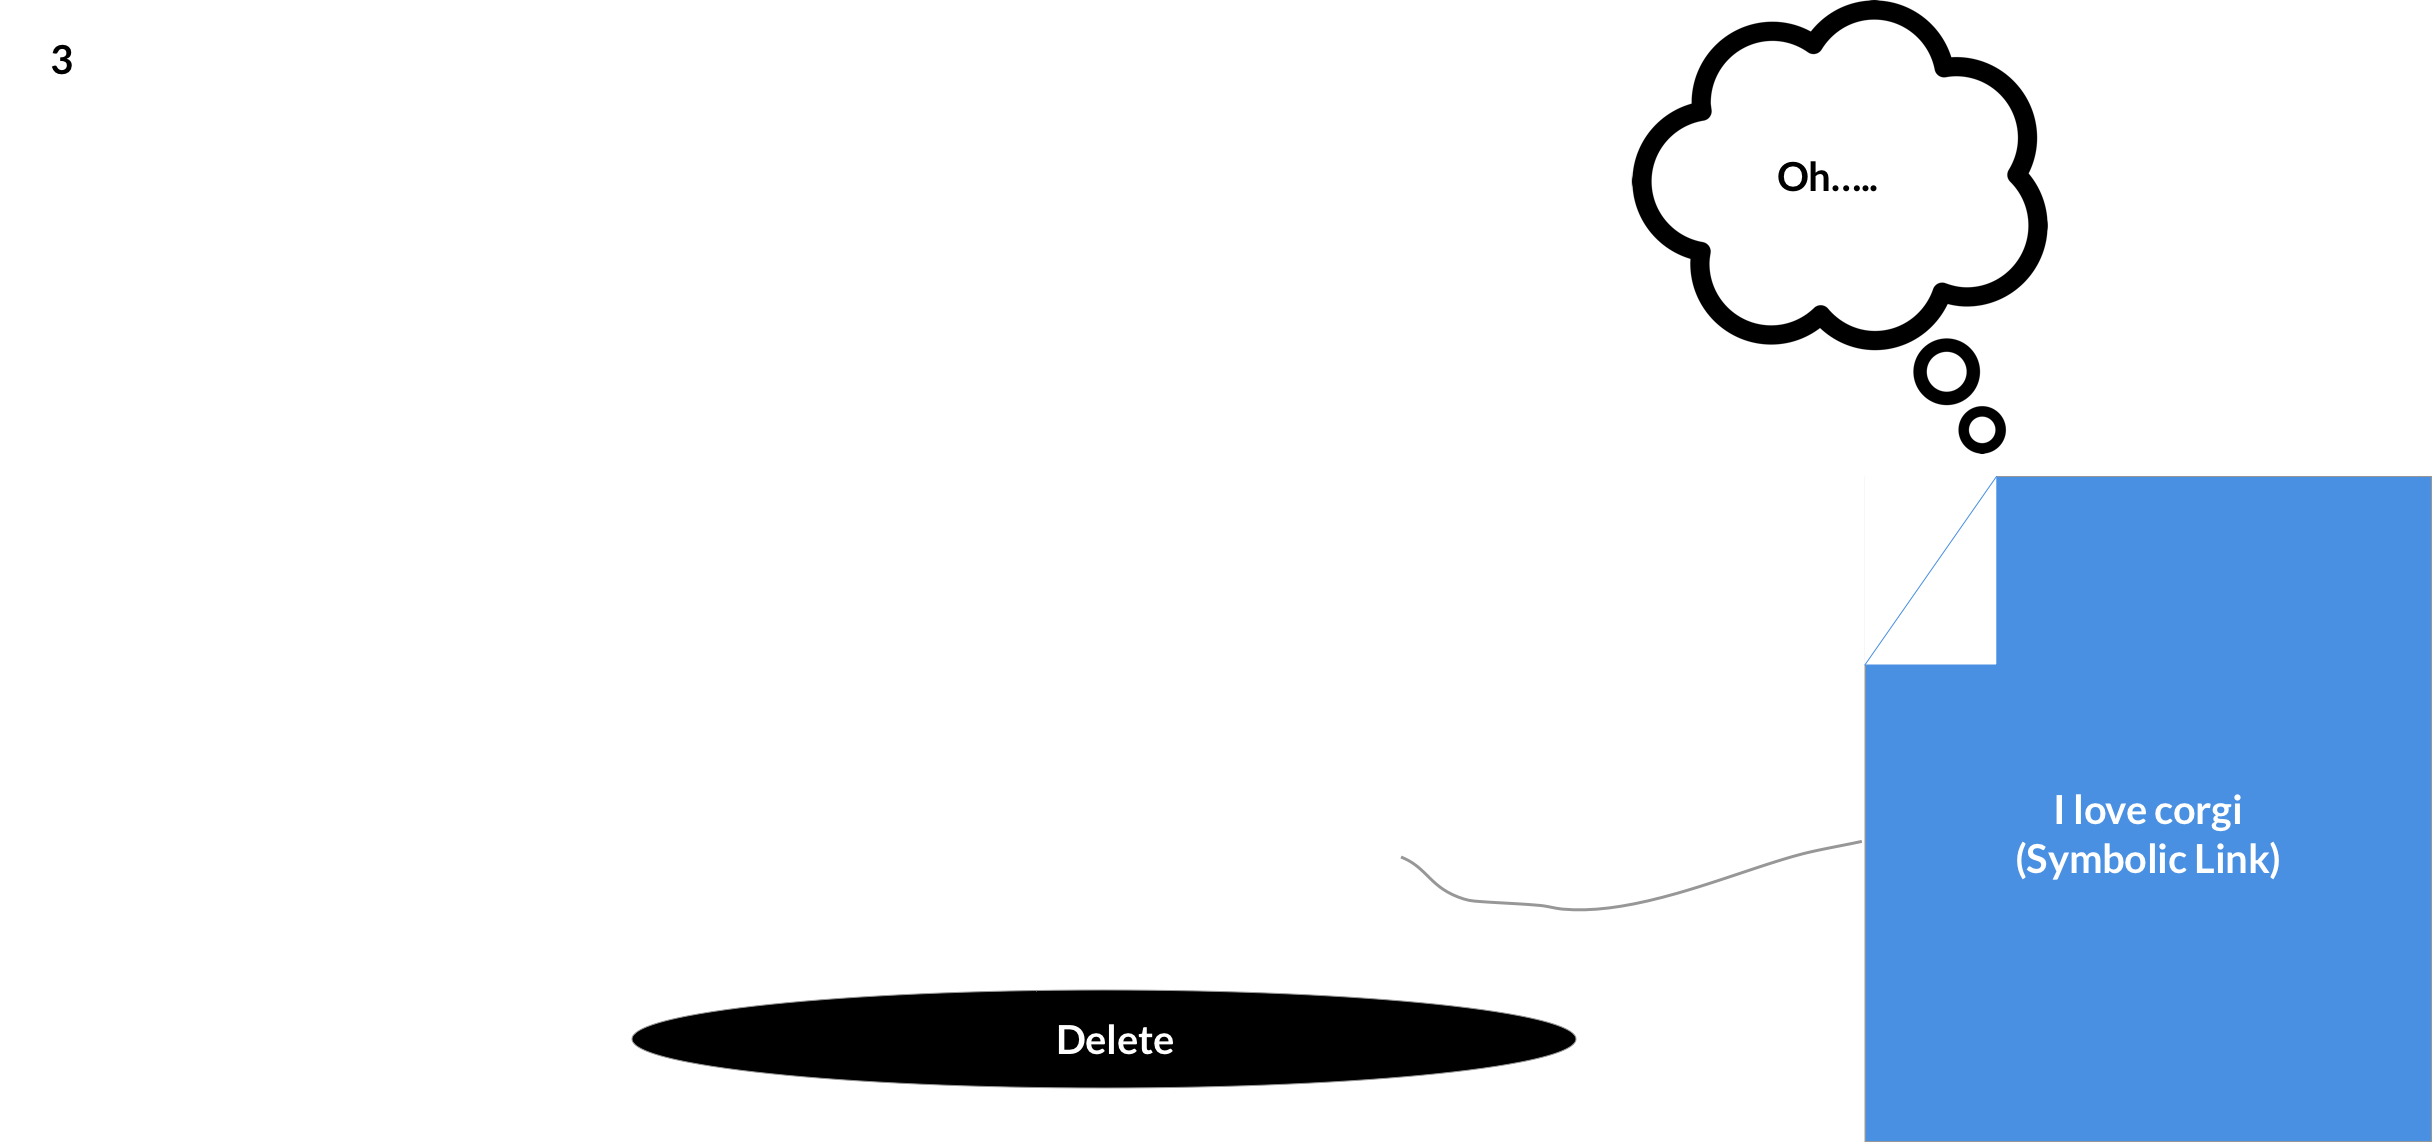
\includegraphics[width=0.8\linewidth]{../images/midterm_4_solution_21.png}
    \end{center}
\end{itemize}

\section{Hard Link:}
\begin{itemize}
    \item \textbf{Syntax:} \texttt{ln \{source\} \{link\}}
    \item Creates a direct reference to inode of a file
    \item Cannot be created to directories (might create cyles)
    \item Cannot create hard links across partitions
    \item Deleting the source file $\to$ No problem
    \begin{itemize}
        \item Inode of file is deleted when reference count is 0
        \item Removing a hard link only removes the file
    \end{itemize}

    \begin{center}
    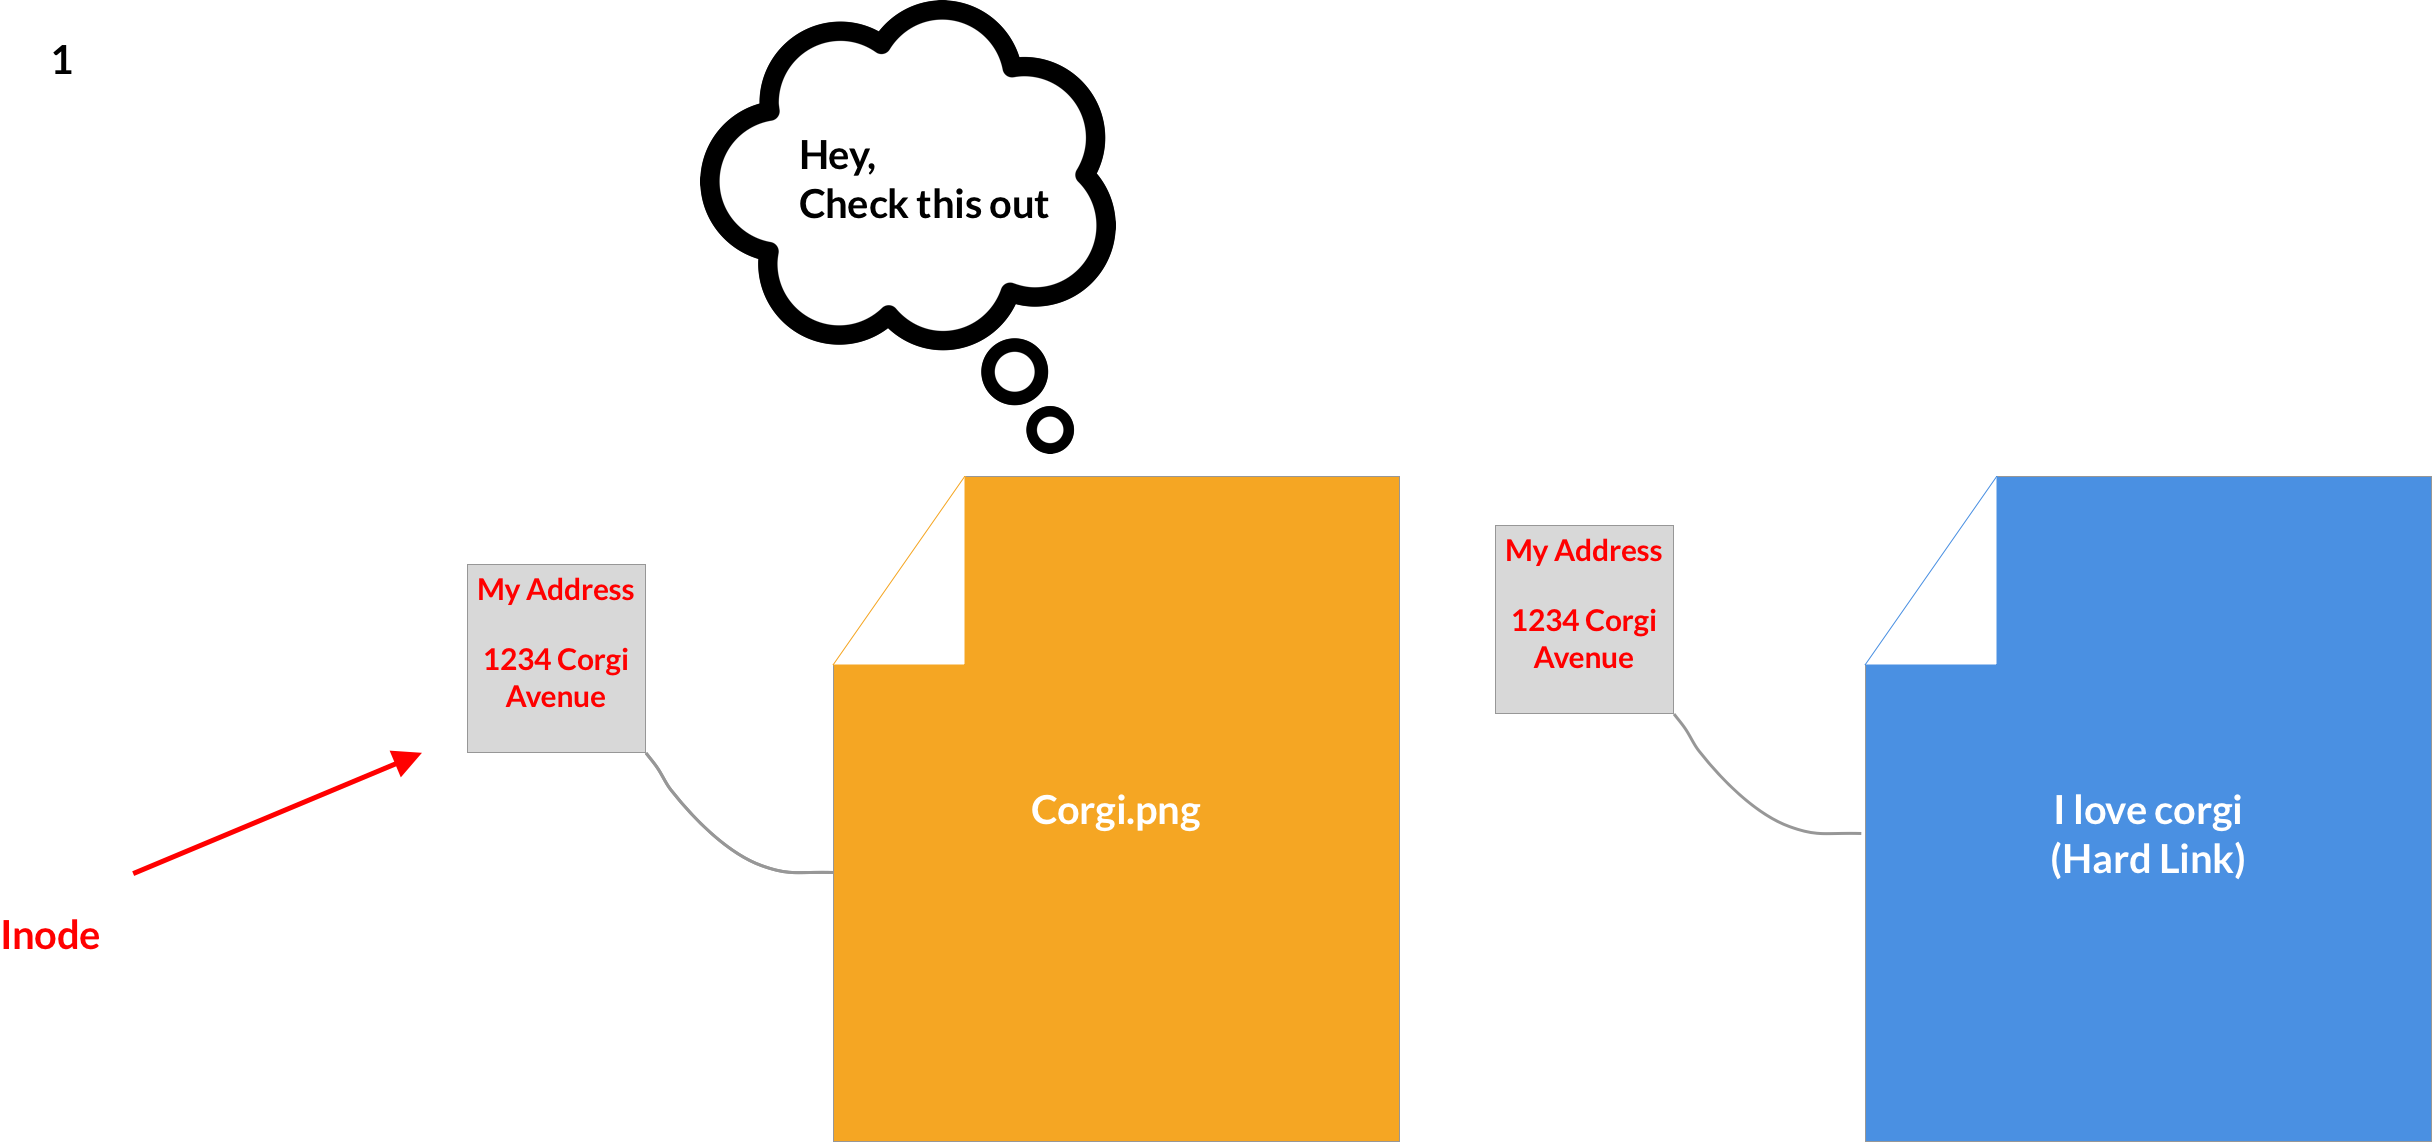
\includegraphics[width=0.8\linewidth]{../images/midterm_4_solution_22.png}
    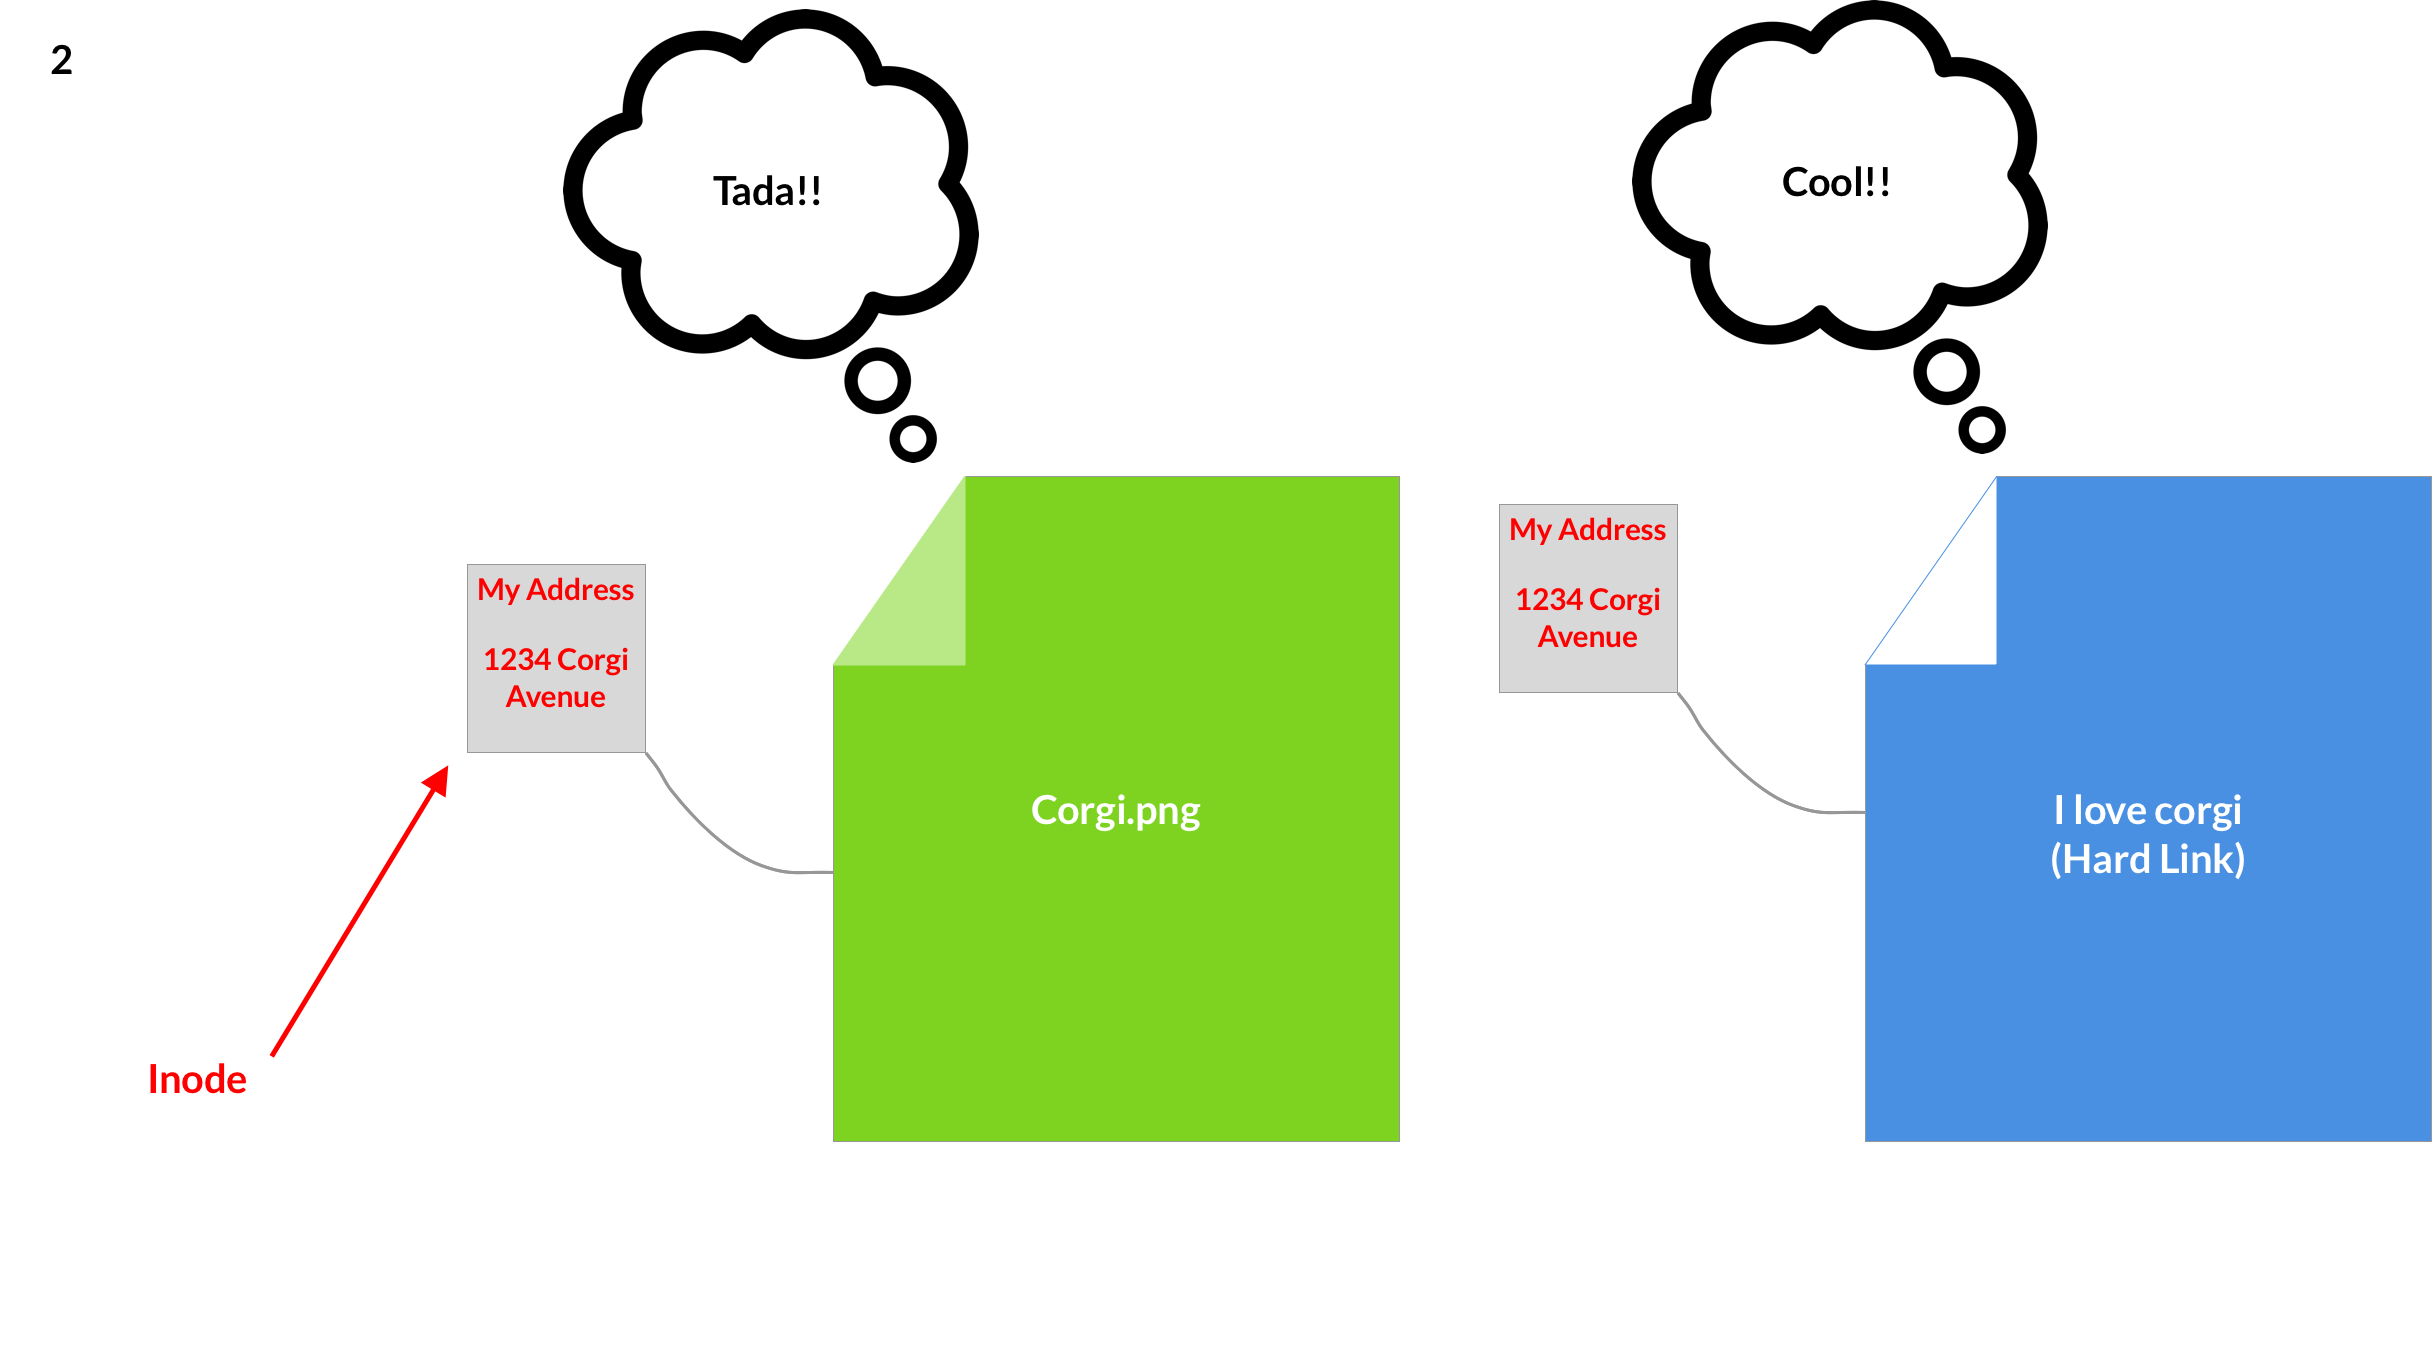
\includegraphics[width=0.8\linewidth]{../images/midterm_4_solution_23.png}
    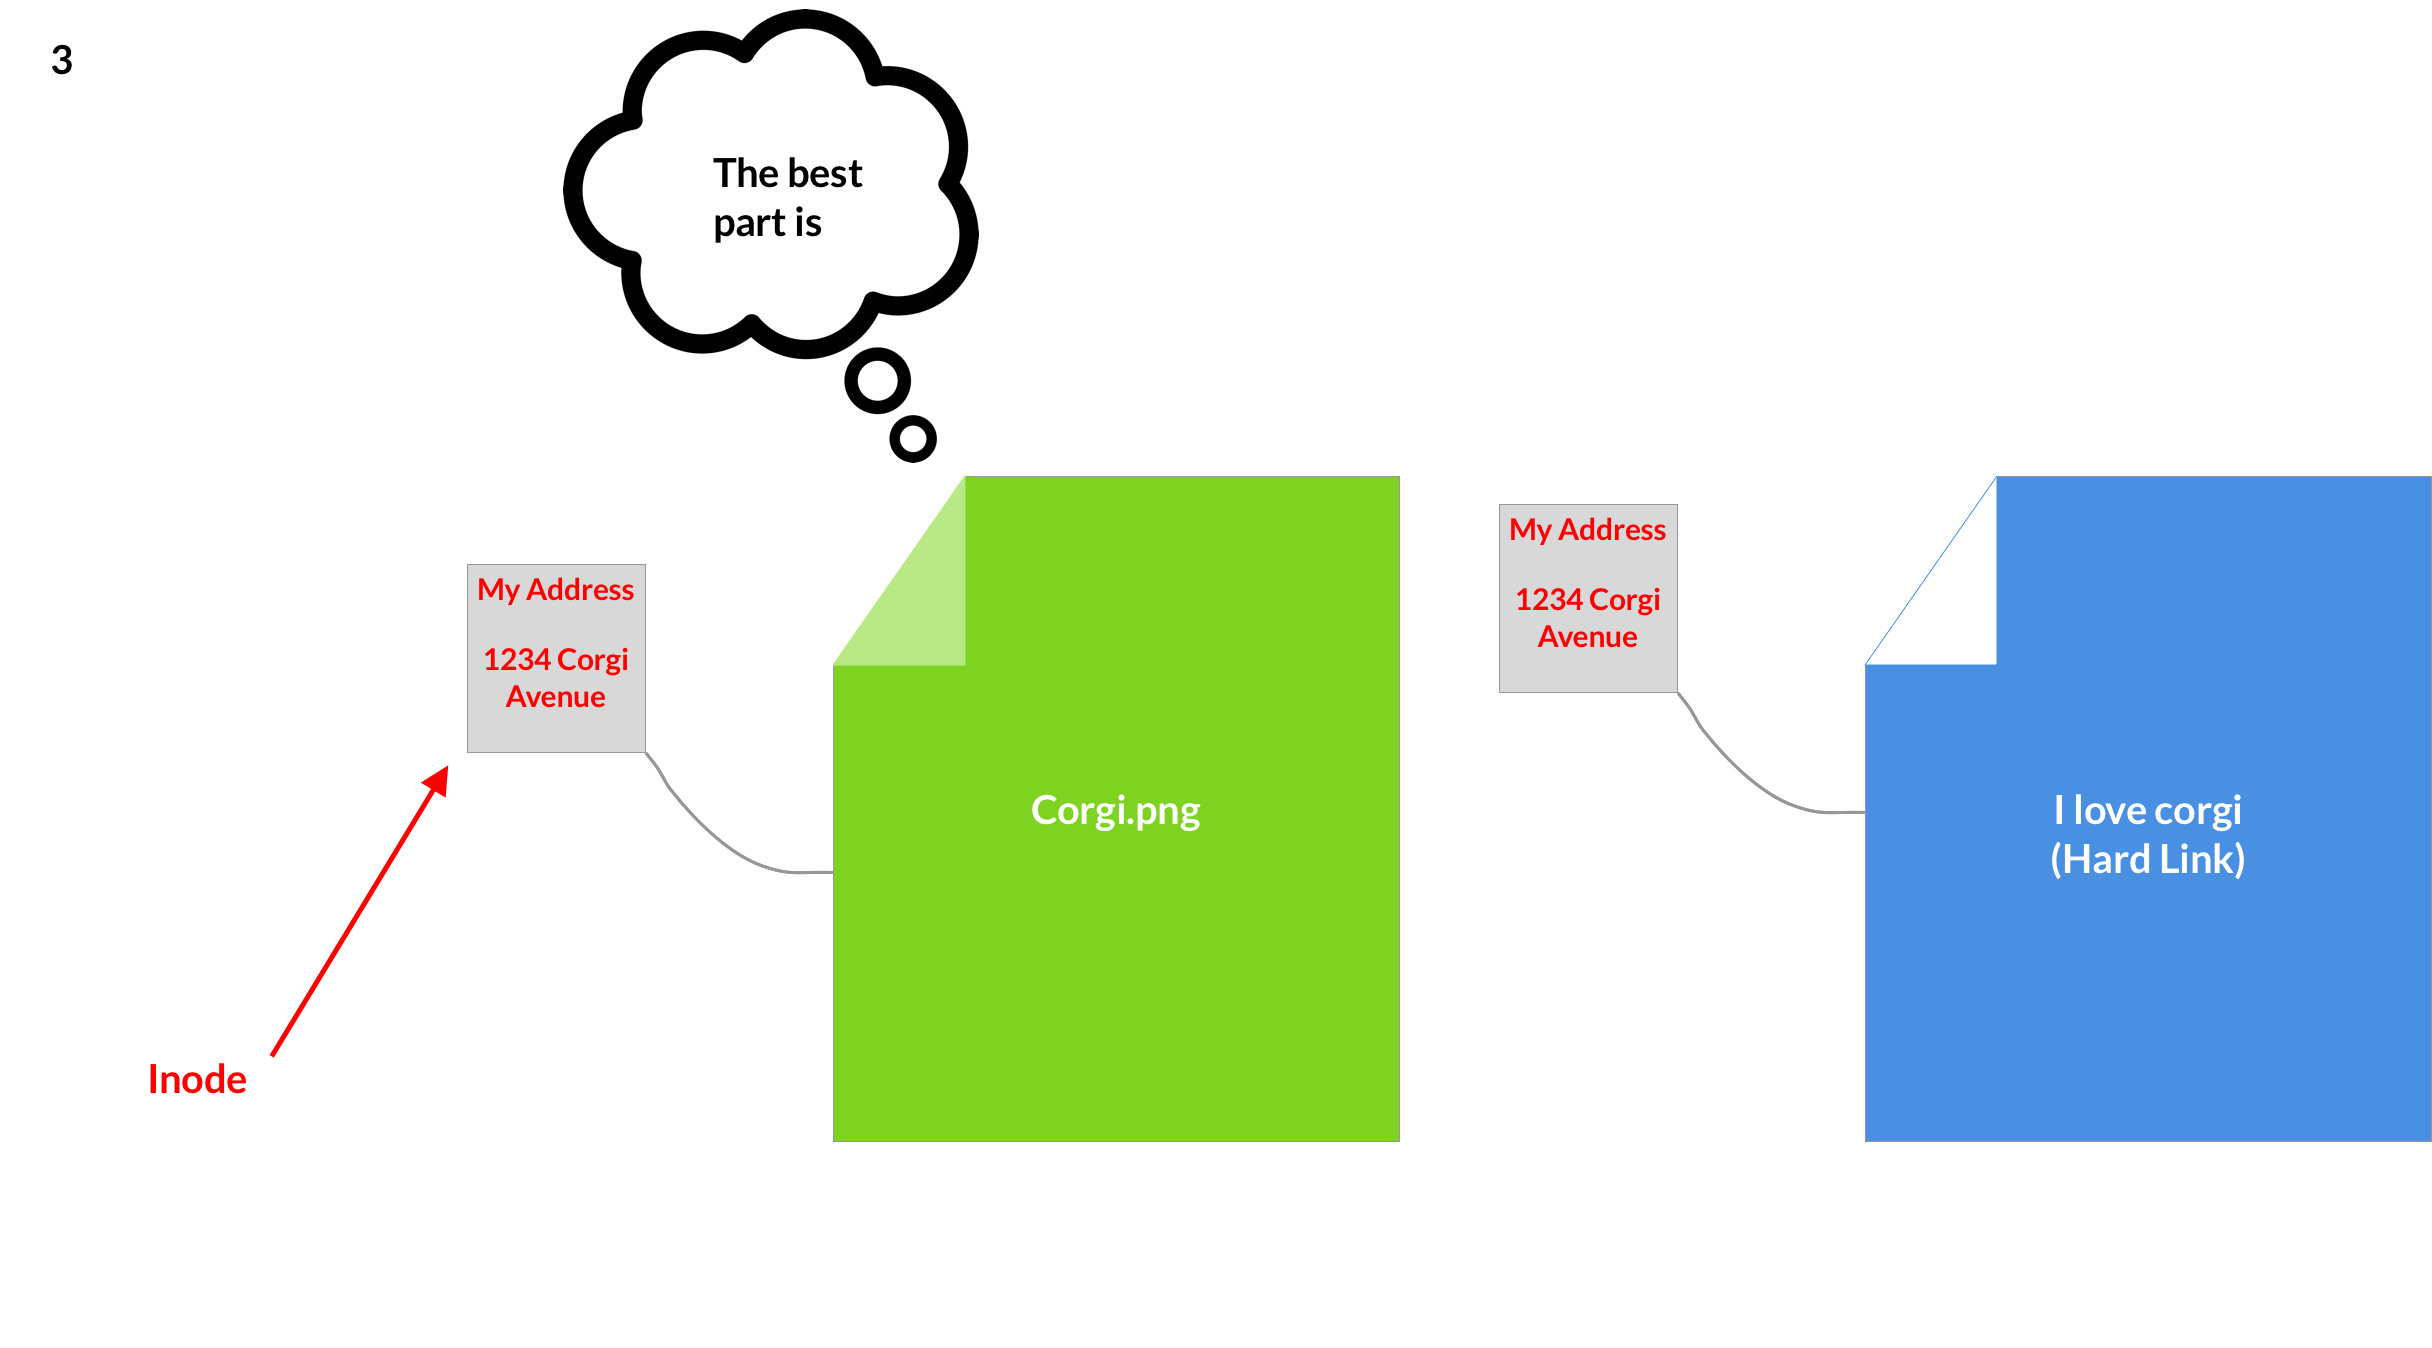
\includegraphics[width=0.8\linewidth]{../images/midterm_4_solution_24.png}
    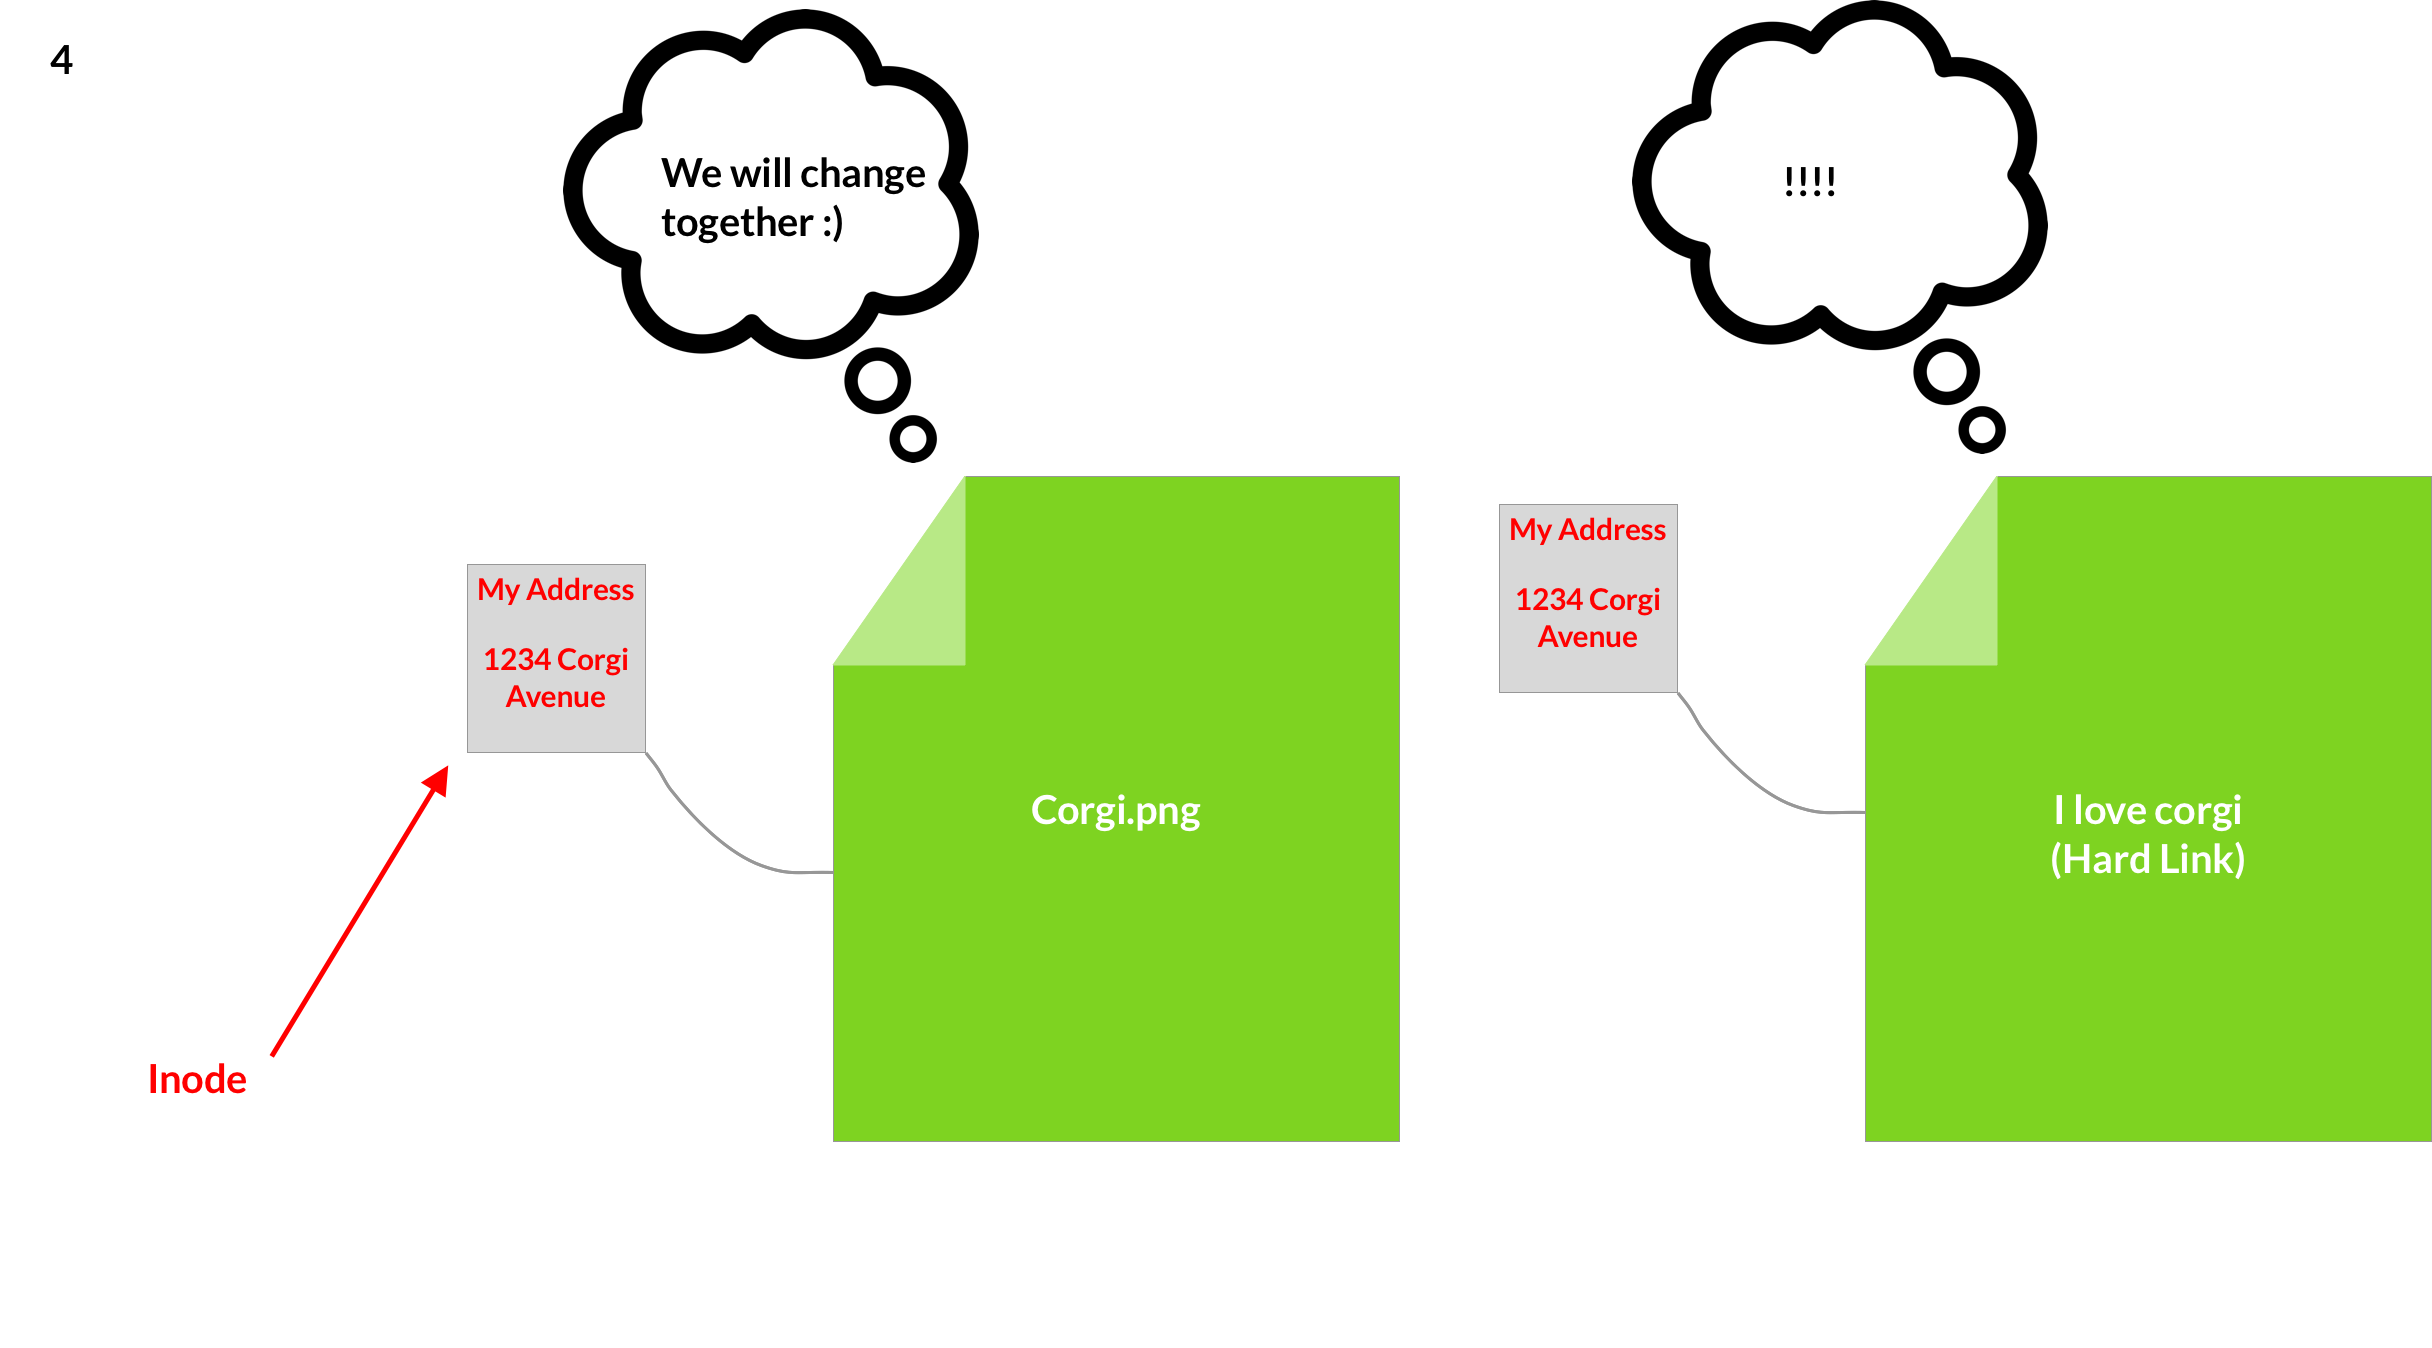
\includegraphics[width=0.8\linewidth]{../images/midterm_4_solution_25.png}
    \end{center}
\end{itemize}

\section{Index-based File System}

\begin{center}
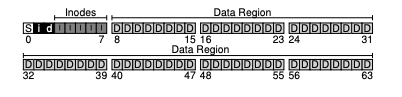
\includegraphics[width=\linewidth]{../images/midterm_2_solution_20.png}
\end{center}

\begin{itemize}
    \item Has following parts

    \begin{itemize}
        \item Superblock
        \item Inode Bitmap
        \item Data Bitmap
        \item Inodes
        \item Data Region
    \end{itemize}

    \item Each block in file system is 4KB
    \item Uses a large amount of metadata per file (especially for large files)
\end{itemize}

\section{Kilobyte}

\begin{itemize}
    \item 1 kilobyte is \underline{1024 bytes}
\end{itemize}

\section{File*}
\begin{itemize}
    \item is an array of bytes which can be created, read, written and deleted
    \item low-level name is called \textbf{inode number} or \textbf{i-number}
\end{itemize}

\section{Static Partitioning}

\begin{itemize}
    \item Divides resources into fixed proportion \underline{once}
    \begin{itemize}
        \item e.g. two possible users of memory $\to$ give fraction of memory to one user and
        rest to the other
    \end{itemize}
    \item Advantages
    \begin{itemize}
        \item Ensures each user receives some share of the resource
        \item Delivers more predictable performance (usually)
        \item Easier to implement
    \end{itemize}
    \item Disadvantages
    \begin{itemize}
        \item Is wasteful
        \item
    \end{itemize}
\end{itemize}


\section{Dynamic Partitioning}

\begin{itemize}
    \item Gives out different amounts of resources over time
    \item Lets resource-hungry users consume idle resources
    \item Advantages
    \begin{itemize}
        \item Flexible
        \item Can achieve better utilization than \textbf{static partitioning}
    \end{itemize}
    \item Disadvantages
    \begin{itemize}
        \item More complex to implement
        \item Could lead to worse performance
        \begin{itemize}
            \item e.g idle resource got consumed by others and take long
            time to reclaim it when needed (the perodic frozen feeling when loading screen)
        \end{itemize}
    \end{itemize}
\end{itemize}

\section{External Fragmentation}

\begin{itemize}
    \item Is various free holes that are generated in either your
    memory or disk space. $^{[8]}$
    \item Are available for allocation, but may be too small to be of
    any use $^{[8]}$
\end{itemize}

\section{Internal Fragmentation}

\begin{itemize}
    \item Is wasted space within each allocated block $^{[8]}$
    \item Occurs when more computer memory is allocated than is needed
\end{itemize}

% \section{Old UNIX File system}
% \begin{itemize}
%     \item was simple, and looked like the following on disk

%     \begin{center}
%     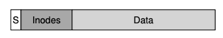
\includegraphics[width=0.6\linewidth]{../images/midterm_2_solution_26.png}
%     \end{center}
%     \item has terrible performance
%     \item suffers from \textbf{external fragmentation}
%     \item had small data block (512 bytes) and transfer of data took too long
% \end{itemize}


\section{Disk Layout Strategies}

\subsection{Index-Based Allocation}
\begin{center}
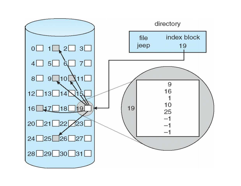
\includegraphics[width=0.6\linewidth]{../images/midterm_4_solution_29.png}
\end{center}

\begin{itemize}
    \item File metadata stored in inode
    \item Has 15 blocks of pointers
    \begin{itemize}
        \item First 12 are direct block pointers
        \item 13th is a single indirect block pointer
        \begin{itemize}
            \item Address of block containing address of data blocks
        \end{itemize}
        \item 14th is a double indirect block pointer
        \begin{itemize}
            \item Address of block containing address of single indirect blocks
        \end{itemize}
        \item 15th is a triple indirect block pointer
        \begin{itemize}
            \item Address of block containing address of double indirect blocks
        \end{itemize}
    \end{itemize}
    \item Index block contains pointers to many other blocks
    \item Advantages
    \begin{itemize}
        \item No external fragmentation
        \item Handles random access better
        \item Files can be easily grown
    \end{itemize}
    \item Disadvantage
    \begin{itemize}
        \item May reuiqre multiple, linked index blocks
    \end{itemize}
\end{itemize}

\bigskip

\underline{\textbf{Example}}

\bigskip

Linux's ext2, ext3

\subsection{Contiguous-Based Allocation}

\begin{center}
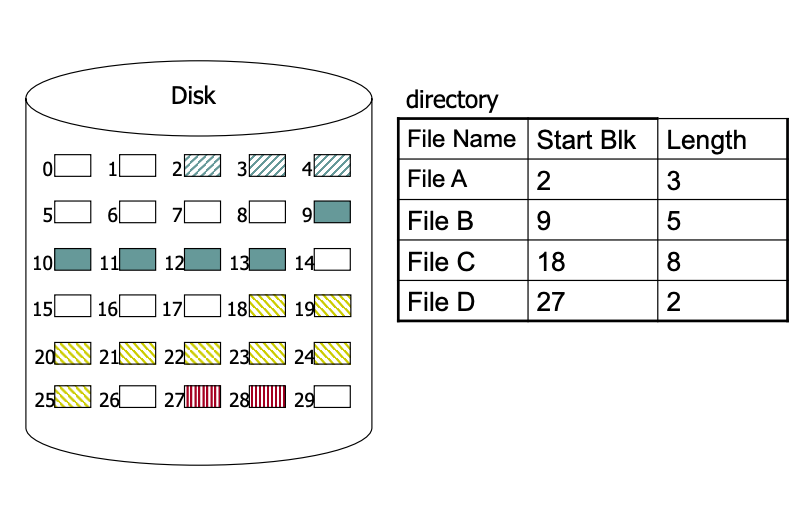
\includegraphics[width=\linewidth]{../images/midterm_2_solution_32.png}
\end{center}

\begin{itemize}
    \item \textbf{Inode} stores starting block and total length
    \item Is simply a disk pointer plus a length (in blocks)
    \begin{itemize}
        \item Together, is called \textbf{extent}
    \end{itemize}
    \item Often allows more than one extent
    \begin{itemize}
        \item resolve problem of finding continuous free blocks
    \end{itemize}
    \item Inode stores starting block and total length
    \item Is less flexible but more compact
    \item Works well when there is enough free space on the disk and files can be laid out contiguously

    \bigskip

    \underline{\textbf{Example}}

    \bigskip

    Linux's ext 4

    \item Advantage

    \begin{itemize}
        \item Is simple
        \begin{itemize}
            \item Finding data block = beginning of data block + length
        \end{itemize}
        \item Fast, simplifies directory access and allows indexing
    \end{itemize}

    \item Disadvantage
    \begin{itemize}
        \item Growing file size could cause problems
        \item Inflexible, causes \textbf{external fragmentation}
        \item Requires compaction
    \end{itemize}
\end{itemize}

\subsection{Linked Allocation}

\begin{center}
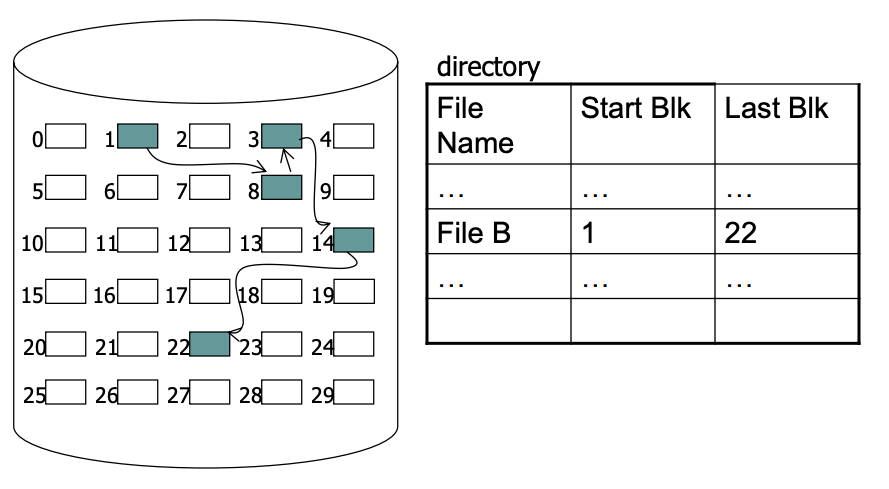
\includegraphics[width=\linewidth]{../images/midterm_4_solution_47.png}
\end{center}

\begin{itemize}
    \item \textbf{Inode} stores the starting block and last block in the directory
    \item Each block in file contains a pointer to the next block
    \item Disadvantage
    \begin{itemize}
        \item If one of the data becomes corrupted, we lost pointers to rest of file
        \item O(n) to find/read nth block (Takes really long time)
    \end{itemize}

    \bigskip

    \underline{\textbf{Example}}

    \bigskip

    Windows' FAT file system

    \bigskip
\end{itemize}

\section{File System Implementation}

\section{Superblock}

\begin{center}
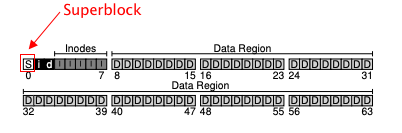
\includegraphics[width=\linewidth]{../images/midterm_2_solution_21.png}
\end{center}

\begin{itemize}
    \item Contains information about the following
    \begin{itemize}
        \item The number of inodes and data blocks in a particular file system
        \item The magic number of some knd to identify the file system type
        \item Where the inode table begins
    \end{itemize}

    \item Is read first on mount before attaching to file system
\end{itemize}


\subsection{Inode/Data bitmap}

\begin{center}
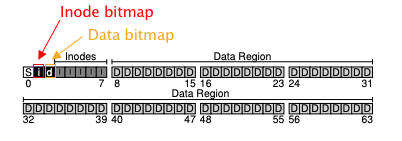
\includegraphics[width=\linewidth]{../images/midterm_2_solution_22.png}
\end{center}

\begin{itemize}
    \item Accessed only when allocation/deallocation is needed
    \begin{itemize}
        \item \texttt{Read()} $\to$ no bitmap required
    \end{itemize}
    \item Uses bit to indicate whether the corres object/block is free
    \begin{itemize}
        \item 0 means free
        \item 1 means in use
    \end{itemize}
\end{itemize}

\subsection{Inode}

\begin{center}
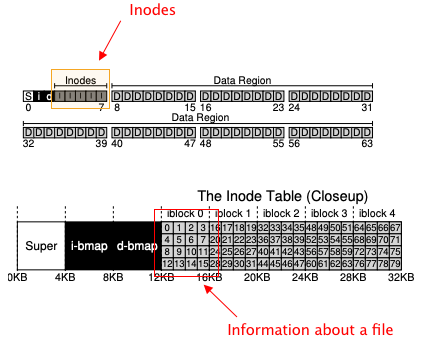
\includegraphics[width=\linewidth]{../images/midterm_2_solution_23.png}
\end{center}

\begin{itemize}
    \item Is a short form for \textbf{index node}
    \item Has a low-level name called \textbf{i-number}
    \begin{itemize}
        \item File also has a low-level named of \textbf{i-number}
        \item File is an inode
    \end{itemize}
    \item Contains all the information you need about a file (i.e. metadata)

    \begin{itemize}
        \item File Type
        \begin{itemize}
            \item e.g. regular file, directory, etc
        \end{itemize}
        \item Size
        \item Number of blocks allocated to it
        \item Protection information
        \begin{itemize}
            \item such as who owns the file, as well as who can access it
        \end{itemize}
        \item Time information
        \begin{itemize}
            \item e.g. When file was created, modified, or last accessed
        \end{itemize}
        \item Location of data blocks reside on disk
    \end{itemize}

    \item total size may vary
    \item inode pointer has size of 4 byte
    \item Has 12 \textbf{direct pointers} to 4KB data blocks
    \item Has 1 \textbf{indirect pointer} [when file grows large enough]
    \item Has 1 \textbf{double indirect Pointer} [when file grows large enough]
    \item Has 1 \textbf{triple indirect Pointer} [when file grows large enough]

    \item Inode before update

    \begin{center}
    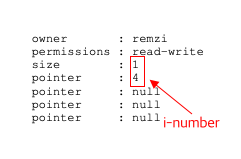
\includegraphics[width=0.6\linewidth]{../images/midterm_4_solution_26.png}
    \end{center}

    \item Inode after update

    \begin{center}
    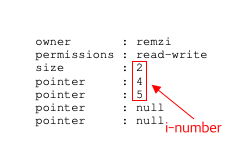
\includegraphics[width=0.6\linewidth]{../images/midterm_4_solution_27.png}
    \end{center}

    % \item Inode block computation

    % \begin{align}
    % \texttt{block number} = (\texttt{inode \#} * \texttt{sizeof(inode)}) / \texttt{block size}
    % \end{align}

    % \bigskip

    % \underline{\textbf{Example}}

    % \bigskip

    % Target: inode \#32

    % Inode Size: 256 bytes

    % Block Size: 4096 bytes

    % \bigskip

    % \begin{align}
    % \texttt{block number} &= (\texttt{inode \#} * \texttt{sizeof(inode)}) / \texttt{block size}\\
    % &= \frac{32 * 256}{4096}\\
    % &= 2
    % \end{align}
\end{itemize}

\section{Data Block}

\begin{itemize}
    \item Size of each block is 4KB
\end{itemize}

\subsection{Indirect Pointers}

\begin{itemize}
    \item Is allocated to data-block if file grows large enough
    \item Has total size of 4 KB or 4096 bytes
    \item Has $4096/4 = 1024$ pointers
    \item Each pointer points to 4KB data-block
    \item File can grow to be $(12 + 1024) \times 4\text{K} = 4144\text{KB}$
\end{itemize}

\subsection{Double Indirect Pointers}

\begin{itemize}
    \item is allocated when single indirect pointer is not large enough
    \item each pointer in first pointer block points to another pointer block
    \item has $1024^2$ pointers
    \item each of $1024^2$ pointers point to 4KB data block
    \item File can grow to be $(12 + 1024 + 1024^2) \times 4\text{K} = 4198448\text{KB}$ or $\approx 4.20 \text{GB}$

    \begin{center}
    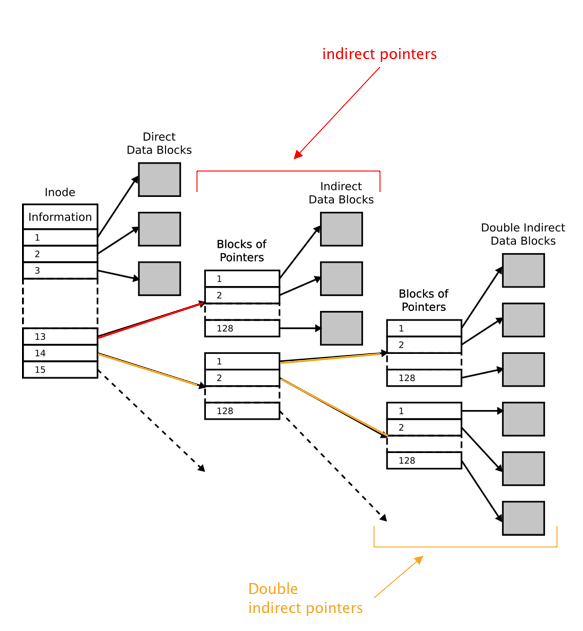
\includegraphics[width=\linewidth]{../images/midterm_2_solution_25.png}
    \end{center}
\end{itemize}

\subsection{Triple Indirect Pointers}

\begin{itemize}
    \item is allocated when double indirect pointer is not large enough
    \item has $1024^3$ pointers
    \item each of $1024^3$ pointers point to 4KB data block
    \item File can grow to be $(12 + 1024 + 1024^2 + 1024^3) \times 4\text{K} = 4299165744\text{KB}$ or $\approx 4.00 \text{TB}$
\end{itemize}

\subsection{Reading a File from Disk}

\underline{\textbf{Example}}

\bigskip

When

\bigskip

\texttt{open("/foo/bar", O\_READONLY)}

\bigskip

is called

\bigskip

\begin{itemize}
    \item the goal is to find the inode of the file \texttt{bar} to read its basic information
    (i.e. includes permission, information, file size etc)
    \item done by traversing the pathname and locate the desired inode
    \item Steps

    \begin{enumerate}[1.]
        \item Find \textbf{inode} of the root directory by looking for \textbf{i-number} (or
        \textbf{inode number})
        \begin{itemize}
            \item Root directory has no parent directory
            \item Root directory's \textbf{inode number} is 2 (for UNIX file systems)
        \end{itemize}

        \item Read the \textbf{inode} of root directory
        \item Once its \textbf{inode} is read, read through its directory data (pointers to \textbf{data blocks})
        until the inode number of \texttt{foo} is found (e.g 42)
        \item Recursively traverse the pathname until the desired inode is found (more specifically, the \textbf{inode number} of bar)
        \item Issue a \texttt{open()} to read \texttt{bar}'s inode to memory
        \item Issue a \texttt{read()} system call to read from file \texttt{bar}

        \begin{itemize}
            \item without \texttt{lseek()}, reads file from the first file data block (e.g. \texttt{bar data[0]})
            \item \texttt{lseek(..., offset\_amt * size\_of\_file\_block)} is used to offset/move to desired block in \texttt{bar}
        \end{itemize}

        \item Trasnfer data to \texttt{buf} data block

        \item Read until \texttt{read()} returns 0, or desired data block has been read
        \item Close \texttt{fd}. No I/O is read.
    \end{enumerate}
\end{itemize}

\subsection{Writing to Disk}

\begin{center}
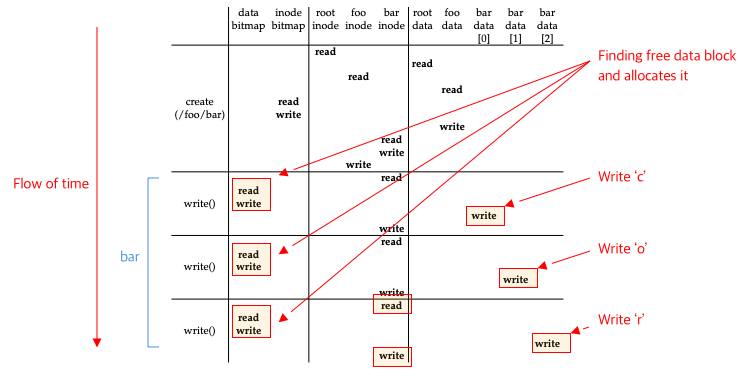
\includegraphics[width=\linewidth]{../images/midterm_4_solution_30.png}
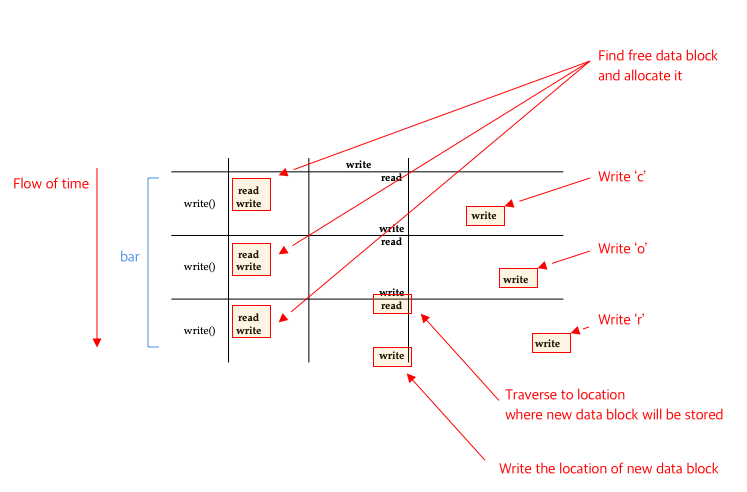
\includegraphics[width=\linewidth]{../images/midterm_4_solution_31.png}
\end{center}

\bigskip

Given a call

\bigskip

\texttt{create(...)} (Note: \texttt{open} to be exact)

\bigskip

\begin{itemize}
    \item 5 I/Os are generated per write

    \begin{itemize}
        \item Read inode (to traverse to the location of new data block)
        \item Reading data bitmap
        \item Writing data bitmap
        \item Write data block
        \item Write inode (to update data block's location in inode)
    \end{itemize}
    \item 10 I/Os are generated per file creation:

    \begin{itemize}
        \item Read inode bitmap (to find free inode)
        \item Write inode bitmap (to mark it allocated)
        \item Create one new inode (to initialize it)
        \item Write the location of new inode block in \texttt{foo} (by linking high-level name of file \texttt{bar} to its inode number and storing in data block)
        \item Perform one read and write to the directory inode and update it
    \end{itemize}
\end{itemize}

\subsection{Static Partitioning}

\begin{itemize}
    \item Divides resources into fixed proportion \underline{once}
    \begin{itemize}
        \item e.g. two possible users of memory $\to$ give fraction of memory to one user and
        rest to the other
    \end{itemize}
    \item Advantages
    \begin{itemize}
        \item Ensures each user receives some share of the resource
        \item Delivers more predictable performance (usually)
        \item Easier to implement
    \end{itemize}
    \item Disadvantages
    \begin{itemize}
        \item Is wasteful
        \item
    \end{itemize}
\end{itemize}

\subsection{Dynamic Partitioning}

\begin{itemize}
    \item Gives out different amounts of resources over time
    \item Lets resource-hungry users consume idle resources
    \item Advantages
    \begin{itemize}
        \item Flexible
        \item Can achieve better utilization than \textbf{static partitioning}
    \end{itemize}
    \item Disadvantages
    \begin{itemize}
        \item More complex to implement
        \item Could lead to worse performance
        \begin{itemize}
            \item e.g idle resource got consumed by others and take long
            time to reclaim it when needed (the perodic frozen feeling when loading screen)
        \end{itemize}
    \end{itemize}
\end{itemize}

\bigskip

\underline{\textbf{Example}}

\bigskip

Linux's ext4 file system

\section{Fields}

\begin{itemize}
    \item Is the members in a structure

    \bigskip

    \begin{center}
    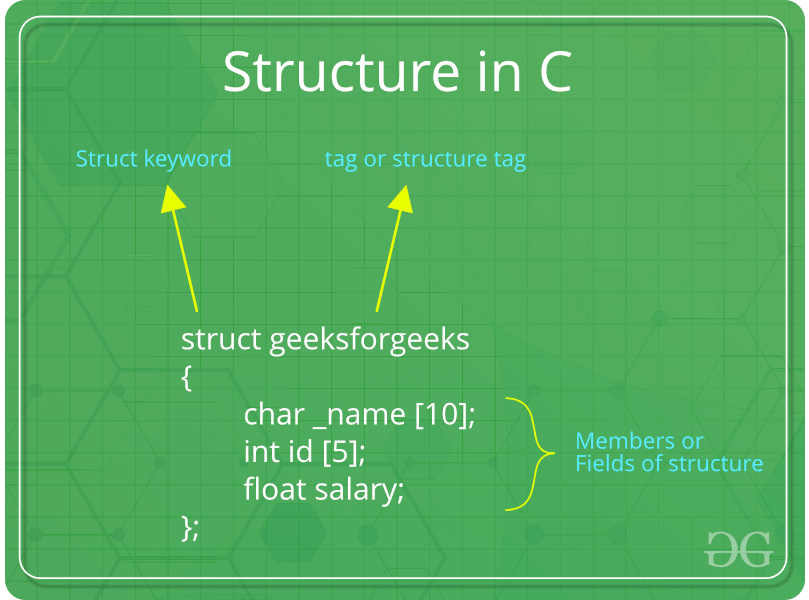
\includegraphics[width=0.6\linewidth]{../images/midterm_2_solution_33.png}
    \end{center}
\end{itemize}

\section{Fast File System}

\begin{itemize}
    \item Modern file system has same APIS (\texttt{read()}, \texttt{write()}, \texttt{open()}, \texttt{close()})
    \item Divides inode/bitmap tables into chunks and stores in different \textbf{cylinder groups}

    \begin{center}
    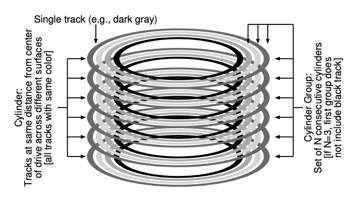
\includegraphics[width=0.8\linewidth]{../images/midterm_2_solution_28.png}
    \end{center}
    \item Each \textbf{block group} or \textbf{cylinder group} is consecutive
    portion of disk's address

    \begin{center}
    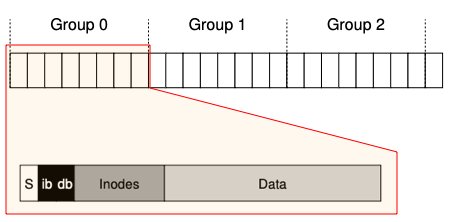
\includegraphics[width=0.8\linewidth]{../images/midterm_2_solution_29.png}
    \end{center}
    \item Advantages
    \begin{itemize}
        \item No external fragmentation
    \end{itemize}
    \item Disadvantages
    \begin{itemize}
        \item Extra overhead: creates and updates many intermediary files (inode, data block) during a write
    \end{itemize}
\end{itemize}

\subsection{FFS Policies: Allocating Files and Directories}

\begin{itemize}
    \item Basic Idea: keep related stuff together, and keep related stuff
    far apart
    \item Directories Step

    \begin{enumerate}[1)]
        \item Find the \textbf{cylinder group} with a low number of allocated directories
        and a high number of free inodes

        \begin{itemize}
            \item low number of allocated directories $\to$ to balance directories
            across groups
            \item high number of free nodes $\to$ to subsequently be able to allocate a bunch offiles
        \end{itemize}
        \item Put directory data and inode to the \textbf{cylinder group}
    \end{enumerate}

    \item Files Step

    \begin{enumerate}[1)]
        \item Allocate the data blocks of a file in the same \textbf{cylinder group} as its inode
        \item Place all files in the same directory in the cylinder group of the directory they are in

        \bigskip

        \underline{\textbf{Example}}

        \bigskip

        On putting \texttt{/a/c}, \texttt{/a/d}, \texttt{/b/f}, FFS would place

        \begin{itemize}
            \item \texttt{/a/c}, \texttt{/a/d} as close as possible in the same \textbf{cylinder group},
            \item \texttt{/b/f} located far away (in some other \textbf{cylinder group})
        \end{itemize}
    \end{enumerate}
\end{itemize}

\section{Log Structured File System}
\begin{itemize}
    \item Wait. This sounds very similar to \textbf{extent-based file system}
    \item Buffers all updates (including metadata) in an in-memory \textbf{segment},
    and when segment is full, it is written to disk in one long, sequential
    transfer to unused part of the disk
    \item Instead of overwriting files, always writes unused
    portion of the disk, and reclaim the old space through cleaning

    \item Motivations
    \begin{enumerate}[1.]
        \item \textbf{System memories are growing}
        \begin{itemize}
            \item Data is cached in memory
            \item Reads are serviced by cache
            \item Disk traffic is increasingly consists of writes
            \item File performance $\approx$ write performance
        \end{itemize}
        \item \textbf{There is a large gap between random I/O performance and
        sequential I/O performance}
        \begin{itemize}
            \item More bits stored on hard drive $\Rightarrow$ bandwith of acessing bits $\uparrow$
            \item Harder to create cheap, small motors that spin platters faster, and move arm more quickly
        \end{itemize}
        \item \textbf{Existing file systems perform poorly on many common workloads}
        \begin{itemize}
            \item Many intermediary writes performed per data block (e.g. Bitmap, inode, data block)
            \item Many short seeks + rotation delays = performance less than the peak
        \end{itemize}
        \item \textbf{File systems are not raid aware}
    \end{enumerate}

    \item How it works (Writing to Disk)

    \bigskip

    Basic idea: Write all updates (e.g. data blocks inodes) to the
    disk sequentially (\textbf{write buffering})

    \bigskip

    \begin{enumerate}[1.]
        \item Buffer updates in an in-memory \textbf{segment}
        \item Write the \textbf{segment} all at once sequentially when received sufficient number of updates
    \end{enumerate}

    \item Advatages

    \begin{enumerate}[1.]
        \item Has very high performance
    \end{enumerate}

    \item Disadvantages

    \begin{enumerate}[1.]
        \item Is complex
        \item Generates lots of garbages
        \item Scattered old data. Needs to run \textbf{compaction} periodically $^{[2]}$
    \end{enumerate}
\end{itemize}

\section{Crash Consistency Problem: File System Checker}

\begin{itemize}
    \item Desired: \textbf{atomic} updates. That is, on crash,
    the file on write is either in (state 1 - before the file got updated)
    or (state 2 - after the file got updated)
    \item Reality: This is not possible
    \item Is the reason why computers have 'Don't turn off computer' message
\end{itemize}

\subsection{Crash Scenarios}

\begin{center}
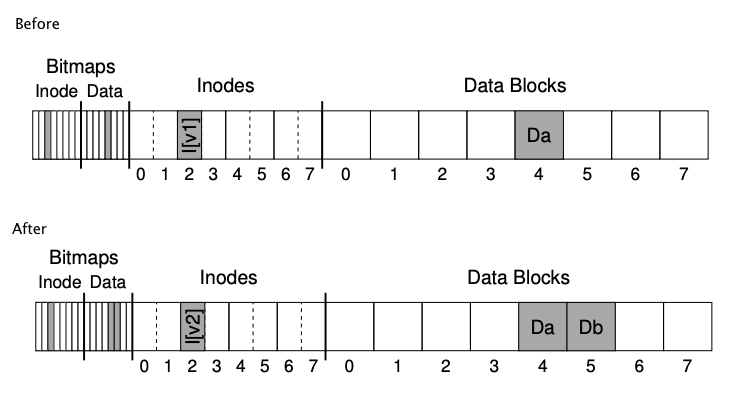
\includegraphics[width=\linewidth]{../images/midterm_2_solution_31.png}
\end{center}


\begin{enumerate}[1)]
    \item Just the data block (Db) is written to disk

    \bigskip

    \begin{itemize}
        \item No inode that points to it
        \item No bitmap that says the block is allocated
        \item It is as if the write never occured
        \item There is no problem here. All is well. (In file system's point of view)
    \end{itemize}

    \bigskip

    \item Just the updated inode (I[v2]) is written to disk

    \bigskip

    \begin{itemize}
        \item Inode points to the disk where \texttt{Db} is about to be written
        \item No bitmap that says the block is allocated
        \item No \texttt{Db} is written
        \item Garbage data will be read
        \item Also creates \textbf{File-system Inconsistency}

        \begin{itemize}
            \item Caused by on-disk bitmap telling us Db 5 is not allocated,
            but inode saying it does
        \end{itemize}
    \end{itemize}

    \bigskip

    \item Just the updated bitmap (B[v2]) is written to disk

    \bigskip

    \begin{itemize}
        \item Bitmap indicates tht block 5 is allocated
        \item No inode exists at block 5
        \item Creates \textbf{file-system inconsistency}
        \item Creates \textbf{space-leak} if left as is

        \begin{itemize}
            \item block 5 can never be used by the file system
        \end{itemize}
    \end{itemize}

    \bigskip

    \item Inode (I[v2]) and bitmap (B[v2]) are written to disk, and not data

    \bigskip

    \begin{itemize}
        \item File system metadata is completely consistent (in perspective of file system)
        \item Garbage data will be read
    \end{itemize}

    \bigskip

    \item Inode (I[v2]) and data block (Db) are written, but not the bit map

    \bigskip

    \begin{itemize}
        \item Creates \textbf{file-system inconsistency}
        \item Needs to be resolved before using file system again
    \end{itemize}

    \bigskip

    \item Bitmap (B[v2]) and data block (Db) are written, but not the inode (I[v2])

    \bigskip

    \begin{itemize}
        \item Creates \textbf{file-system inconsistency} between inode and data bitmap
        \item Creates \textbf{space-leak} if left as is
        \begin{itemize}
            \item Inode block is lost for future use
        \end{itemize}
        \item Creates \textbf{data-leak} if left as is

        \begin{itemize}
            \item Data block is lost for future use
        \end{itemize}
    \end{itemize}
\end{enumerate}

\subsection{File System Checker}

\begin{itemize}
    \item Basic Idea: Let inconsistencies happen and fix them later (when rebooting)
    \item Is used by UNIX tool \textbf{fsck} ('file system checker')
    \item Summary of how it works

    \begin{itemize}
        \item \textbf{Inode State}
        \begin{itemize}
            \item Corruption in file is checked (e.g. does it have valid file type such as directory file, or links)
            \item Solved by removing it, and updating the bitmap if inode cannot be fixed easily
        \end{itemize}
        \item \textbf{Inode links}
        \begin{itemize}
            \item Number of references in each inode is checked
            \item Check is done by reading the entire directory tree and building its own link count
            \item Solved by fixing the count if there is mismatch, or by moving to \texttt{lost+found}
            directory if there is no directory refers to it
        \end{itemize}
        \item \textbf{Duplicates}
        \begin{itemize}
            \item Duplicate pointers (i.e. two different inodes pointing to same block) is checked
            \item Solved by either removing one of two inodes, or creating a copy for each
        \end{itemize}
        \item \textbf{Bad Blocks}

        \begin{itemize}
            \item A pointer that points to something outside is partition is checked
            \item Solved by removing the block
        \end{itemize}

        \item \textbf{Directory Checks}

        \begin{itemize}
            \item Making sure that \texttt{.} and \texttt{..} are first entry is checked
            \item Allocation of inodes referred to in a directory entry is checked
            \item Making sure that no directory is linked more than once is checked
        \end{itemize}
    \end{itemize}

    \item Disadvantage
    \begin{itemize}
        \item Way too slow. May take Hours.
        \item Wasteful (Make mistake once, and check everything)
        \item Doesn't solve all problems (e.g. inode with incorrect data blocks)
    \end{itemize}
\end{itemize}

\section{Journaling}
\begin{itemize}
    \item Is a popular solution to \textbf{crash-consistency problem}
    \item Many file systems use this idea (e.g. ext3, ext4, windows NTFS)
    \item Basic idea

    \begin{itemize}
        \item before overwriting the structures in place, write down
        (in a well-known location) a little note of what you are about to do
        \item If crash occurs, read note and try again
    \end{itemize}

    \bigskip

    \begin{center}
    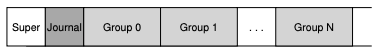
\includegraphics[width=0.8\linewidth]{../images/midterm_4_solution_34.png}
    \end{center}

    \item Advantage

    \begin{itemize}
        \item Greatly reduces amount of work required during recovery
    \end{itemize}
\end{itemize}

\subsection{Transaction Beginning (TxB)}
\begin{itemize}
    \item Where does computer read update instruction (journal ? journal superblock ?)?
    \item In data Journaling, where is comitted data generated and stored prior to putting it in file system?
    \item Includes information about current update
    \item Contains \textbf{Transaction Identifier} or TID
\end{itemize}

\subsection{Transaction End (TxE)}
\begin{itemize}
    \item Is marker of the end of transaction
    \item Also contains \textbf{Transaction Identifier} or TID
\end{itemize}

\subsection{Checkpointing}
\begin{itemize}
    \item Act of overwriting of old structure in the file system between
    \textbf{transaction beginning} and \textbf{transaction end}
\end{itemize}

\subsection{Journaling Superblock}

\begin{itemize}
    \item Records information on which transactions have not yet been checkpointed
    \item Oldest and newest non-checkpointed transactions exist here
    \item Is different from file system superblock
\end{itemize}

\subsection{Data Journaling}

\begin{center}
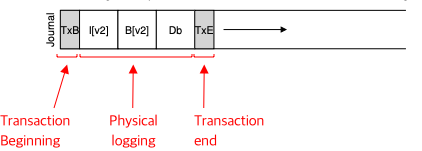
\includegraphics[width=0.8\linewidth]{../images/midterm_4_solution_35.png}
\end{center}

\begin{itemize}
    \item [\color{red}Important\color{black}] Is written to journal before putting onto file system!!!
    \item Steps

    \begin{center}
    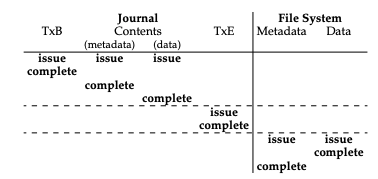
\includegraphics[width=0.8\linewidth]{../images/midterm_4_solution_41.png}
    \end{center}

    \begin{enumerate}[1.]
        \item \textbf{Journal Write}: Write the contents of the transaction (including TxB, metadata and data)
        to log

        \begin{center}
        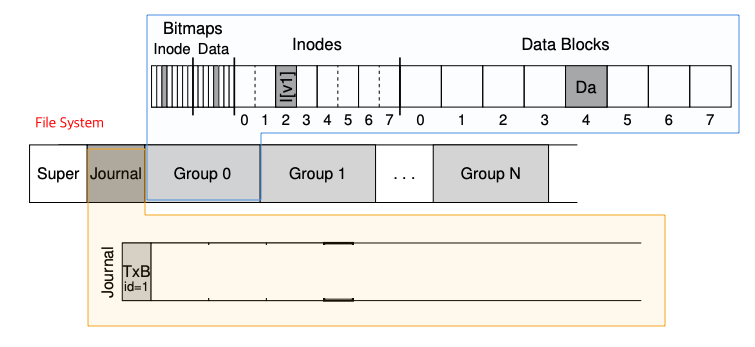
\includegraphics[width=0.8\linewidth]{../images/midterm_4_solution_36.png}
        \end{center}

        \item \textbf{Journal Commit:} Write the transaction commit block (containing TxE) to log; wait wait for write to complete
        \begin{itemize}
            \item After this, transaction is \textbf{committed}
        \end{itemize}

        \begin{center}
        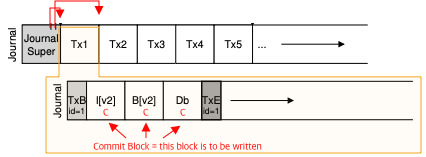
\includegraphics[width=0.8\linewidth]{../images/midterm_4_solution_37.png}
        \end{center}

        \item \textbf{Checkpoint:} Write the contents of the update (metadata and data) to their final on-disk location

        \begin{center}
        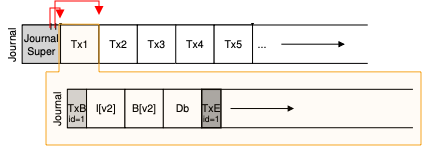
\includegraphics[width=0.9\linewidth]{../images/midterm_4_solution_38.png}
        \end{center}

        \item \textbf{Free:} Mark the transaction free in the journal by updating the
        journal superblock

        \begin{center}
        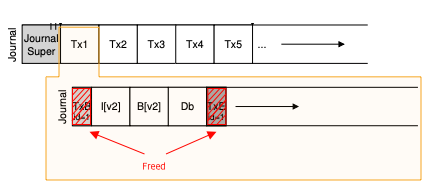
\includegraphics[width=0.8\linewidth]{../images/midterm_4_solution_39.png}
        \end{center}

        \item Repeat until done
    \end{enumerate}

    \item Disadvantage

    \begin{itemize}
        \item Each data block is written twice
    \end{itemize}

    \item Recovery Steps

    \begin{itemize}
        \item Crash at step 1 $\to$ skip pending update
        \item Crash during step 2 and 3 $\to$ replay the update

        \begin{itemize}
            \item Happens during boot
        \end{itemize}
    \end{itemize}
\end{itemize}

\subsection{Metadata Journaling}

\begin{itemize}
    \item Goal: Reduce number of writes
    \item Data block is written to file system first
    \item Metadata (inode and bitmap information) are written to journal before checkpoint
    \item Is order dependent
    \begin{itemize}
        \item e.g. I[v2] and B[v2] make to disk and data block does not
        \item If data block is a garbage data, file-system will assume all is okay
        \item Writing data block first guarentees that a pointer will never point to garbage
    \end{itemize}

    \begin{center}
    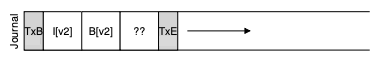
\includegraphics[width=0.8\linewidth]{../images/midterm_4_solution_40.png}
    \end{center}

    \item Steps

    \begin{center}
    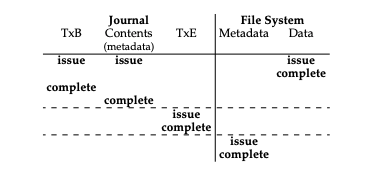
\includegraphics[width=0.8\linewidth]{../images/midterm_4_solution_42.png}
    \end{center}

    \begin{enumerate}[1.]
        \item \textbf{Data Write:} Write data to final location; wait for completion

        \begin{center}
        \includegraphics[width=0.8\linewidth]{../images/midterm_4_solution_43.png}
        \end{center}

        \item \textbf{Journal Metadata Write:} Write the begin block and metadata to the \underline{log};
        wait for writes to complete

        \item \textbf{Journal Commit:} Write the transaction commit block (containing TxE) to
        the log; wait for the write to complete


        \begin{center}
        \includegraphics[width=0.8\linewidth]{../images/midterm_4_solution_44.png}
        \end{center}

        \item \textbf{Checkpoint Metadata:} Write the contents of the metadata update
        to their final locations within the file system

        \begin{center}
        \includegraphics[width=0.8\linewidth]{../images/midterm_4_solution_45.png}
        \end{center}
        \item \textbf{Free:} Mark the transaction free in journal superblock

        \begin{center}
        \includegraphics[width=0.8\linewidth]{../images/midterm_4_solution_46.png}
        \end{center}
    \end{enumerate}
    \item Block Reuse

    \begin{itemize}
        \item Never reuse blocks until checkpointed out of the journal
    \end{itemize}
    \item Advantage
    \begin{itemize}
        \item Solves double write problem in \textbf{data journaling}
    \end{itemize}
\end{itemize}

\end{document}
